\section{Experimental Uncertainties}\label{sec-unc} % TODO there's more info in the main fit part
While efforts are made to correctly simulate the collection and reconstruction of information with the ATLAS detector, inaccuracies permeate this procedure and must be taken into account in the statistical analysis of Section \ref{sec-fitFramework}. Several types of experimental uncertainties are considered in the combined analysis, to cover the systematics effects due to the detector performance, the reconstruction of objects such as leptons and jets, and the effects of flavour tagging. Table \ref{tab:ExpSysts} summarises the various contributions that are sources of uncertainty, which are detailed in this section.

\begin{table}
    \centering
    \renewcommand{\arraystretch}{1.2}
    \resizebox{1.05\textwidth}{!}{%
      \begin{tabular}{llr}
        \hline \hline
        \textbf{Systematic uncertainty name} & $\quad\quad\quad\quad\quad$ \textbf{Description} &\textbf{Regime} \\
        \hline
        \multicolumn{3}{c}{Luminosity and Pile-up}\\
        \hline
        \texttt{LUMI\_2015\_2018 }& Uncertainty on total integrated luminosity & All \\
        \texttt{PRW\_DATASF}& Uncertainty on pile-up modelling & All \\
        \hline
        \multicolumn{3}{c}{\etm and $E_{\text{T,trk}}^{\text{miss}}$}\\
        \hline
        \texttt{MET\_SoftTrk\_ResoPara(Perp)}&  Soft term longitudinal (transverse) resolution uncertainty & All \\
        \texttt{MET\_SoftTrk\_Scale   }&  Soft term scale uncertainty & All \\
        \texttt{MET\_JetTrk\_Scale    }& $E_{\text{T,trk}}^{\text{miss}}$ scale uncertainty & All \\
        \texttt{METTrig\{Stat,Top,Z,Sumpt\}} & Trigger efficiency uncertainty & Resolved \\
        \hline
        \multicolumn{3}{c}{Electrons}\\
        \hline
        \texttt{EL\_EFF\_Trigger\_TOTAL}&  Trigger efficiency uncertainty & All \\
        \texttt{EL\_EFF\_Reco\_TOTAL}&  Reconstruction efficiency uncertainty & All \\
        \texttt{EL\_EFF\_ID\_TOTAL}&  Identification (ID) efficiency uncertainty & All \\
        \texttt{EL\_EFF\_Iso\_TOTAL}&  Isolation efficiency uncertainty & All \\
        \texttt{EG\_SCALE\_ALL}&        Energy scale uncertainty   &  all  \\
        \texttt{EG\_RESOLUTION\_ALL}&    Energy resolution uncertainty  & All \\
        \hline
        \multicolumn{3}{c}{Muons}\\
        \hline
        \texttt{MUON\_EFF\_RECO\_\{STAT,SYS\} }& {Reconstruction and ID efficiency uncertainty for muons with $p_T > 15$ GeV} & All \\
        \texttt{MUON\_EFF\_RECO\_\{STAT,SYS\}\_LOWPT }&{Reconstruction and ID efficiency uncertainty for muons with $p_T \leq 15$ GeV} & All \\
        \texttt{MUON\_EFF\_ISO\_\{STAT,SYS\} }& {Isolation efficiency uncertainty} & All \\
        \texttt{MUON\_EFF\_TTVA\_\{STAT,SYS\} }& {Track-to-vertex association efficiency uncertainty} & All \\
        \texttt{MUON\_SCALE}&    Momentum scale uncertainty & All \\
        \texttt{MUON\_SAGITTA\_RHO(RESBIAS)} & Momentum scale uncertainty to cover charge-dependent local misalignment effects & All \\
        \texttt{MUON\_ID(MS) }& Momentum resolution uncertainty of the inner detector (muon spectrometer) & All \\
        \texttt{MUON\_EFF\_Trig\{Stat,Sys\}Uncertainty} & Trigger efficiency uncertainty & All \\
        \hline
        \multicolumn{3}{c}{Taus}\\
        \hline
        \texttt{TAUS\_TRUEHADTAU\_EFF\_RECO\_TOTAL}& {Reconstruction efficiency} & All \\
        \texttt{TAUS\_TRUEHADTAU\_EFF\_RNNID\_*}& {RNN ID efficiency} & All \\
        \texttt{TAUS\_TRUEHADTAU\_SME\_TES\_*}& {In-Situ tau energy scale correction} & All \\
        \texttt{TAUS\_TRUEELECTRON\_EFF\_ELEBDT\_*}& {Electron Veto efficiency SF} & All \\
        \hline
        \multicolumn{3}{c}{Small-R jets}\\
        \hline
        \texttt{JET\_CR\_BJES\_Response }& Energy scale uncertainties for $b$-jets & All \\
        \texttt{JET\_CR\_EffectiveNP\_Detector\{1-2\} }& Energy scale uncertainties due to in-situ calibration & All \\
        \texttt{JET\_CR\_EffectiveNP\_Mixed\{1-3\} }& Energy scale uncertainties due to in-situ calibration & All  \\
        \texttt{JET\_CR\_EffectiveNP\_Modelling\{1-4\} }& Energy scale uncertainties due to in-situ calibration & All \\
        \texttt{JET\_CR\_EffectiveNP\_Statistical\{1-6\} }& Energy scale uncertainties due to in-situ calibration & All \\
        \texttt{JET\_CR\_EtaIntercal\_Modelling}& Energy scale uncertainties to cover $\eta$-intercalibration non-closure & All \\
        \texttt{JET\_CR\_EtaIntercal\_NonClosure\_highE}& Energy scale uncertainties to cover $\eta$-intercalibration non-closure & All \\
        \texttt{JET\_CR\_EtaIntercal\_NonClosure\_negEta}& Energy scale uncertainties to cover $\eta$-intercalibration non-closure & All \\
        \texttt{JET\_CR\_EtaIntercal\_NonClosure\_posEta}& Energy scale uncertainties to cover $\eta$-intercalibration non-closure & All \\
        \texttt{JET\_CR\_EtaIntercal\_TotalStat}& Energy scale uncertainties to cover $\eta$-intercalibration non-closure & All \\
        \texttt{JET\_CR\_Flav\_Comp(Flavor\_Response) }& Energy scale uncertainty related to flavour composition (response) & All \\
        \texttt{JET\_CR\_PunchTroughMC16 }& Energy scale uncertainty for 'punch-through' & All \\
        \texttt{JET\_CR\_SingleParticle\_HighPt }& Energy scale uncertainty for the behavior of high-\pt\ single hadrons & All \\
        \texttt{JET\_CR\_JER\_DataVsMC}& Energy resolution total uncertainty  & All \\
        \texttt{JET\_CR\_JER\_EffectiveNP\_\{1-6,7restTerm\}}& Energy resolution total uncertainties & All \\
        \texttt{JET\_JvtEfficiency}& JVT efficiency uncertainty  & All \\
        \texttt{JET\_PU\_\{OffsetMu(NPV),PtTerm,RhoTopology\}}& Energy scale uncertainties due to pile-up effects & All \\
        \hline
        \multicolumn{3}{c}{Large-R jets}\\
        \hline
        \texttt{FJ\_JMSJES\_Baseline\_Kin }&  {Energy and mass scale uncertainty due to basic data-simulation differences} & Boosted \\
        \texttt{FJ\_JMSJES\_Modelling\_Kin }& {Energy and mass scale uncertainty due to simulation differences} & Boosted \\
        \texttt{FJ\_JMSJES\_Tracking\_Kin }&  {Energy and mass scale uncertainty on reference tracks} & Boosted \\
        \texttt{FJ\_JMSJES\_TotalStat\_Kin }& {Energy and mass scale uncertainty from stat. unc. on the measurement} & Boosted \\
        \texttt{FJ\_JER }&  Energy resolution uncertainty & Boosted \\
        \texttt{FJ\_JMR }&  Mass resolution uncertainty & Boosted \\
        \hline
        \multicolumn{3}{c}{Flavour tagging: PFlow jets }\\
        \hline
        \texttt{FT\_EFF\_PFlow\_Eigen\_B\_\{0-44\}}& {Tagging efficiency uncertainties for $b$-jets} & Resolved \\
        \texttt{FT\_EFF\_PFlow\_Eigen\_C\_\{0-19\}}&{Tagging efficiency uncertainties for $c$-jets} & Resolved \\
        \texttt{FT\_EFF\_PFlow\_Eigen\_Light\_\{0-19\}}&{Tagging efficiency uncertainties for light-jets} & Resolved \\
        \texttt{FT\_EFF\_PFlow\_extrapolation }& Tagging efficiency uncertainty for high-\pt\ jets & Resolved \\
        \hline
        \multicolumn{3}{c}{$b$-tagging: VR track jets}\\
        \hline
        \texttt{FT\_EFF\_VR\_Eigen\_B\_\{0-4\}}& {$b$-tagging efficiency uncertainties for $b$-jets} & Boosted \\
        \texttt{FT\_EFF\_VR\_Eigen\_C\_\{0-3\}}&{$b$-tagging efficiency uncertainties for $c$-jets} & Boosted \\
        \texttt{FT\_EFF\_VR\_Eigen\_Light\_\{0-3\}}&{$b$-tagging efficiency uncertainties for light-jets} & Boosted \\
        \texttt{FT\_EFF\_VR\_extrapolation }& $b$-tagging efficiency uncertainty for high-\pt\ jets & Boosted \\
        \hline \hline
    \end{tabular}
    }
    \caption{Summary of all experimental systematic uncertainties. }
    \label{tab:ExpSysts}
    \renewcommand{\arraystretch}{1.0}
  \end{table}
   %TODO check that the ftag uncertainties are still completely decorrelated for the VR track and PFlow

\paragraph{Luminosity \& Pile-up:} The measured Run 2 luminosity for ATLAS is 140 fb$^{-1}$ with an uncertainty of 0.83\% \cite{ATLAS:2022hro}. The measurement is performed by $x-y$ beam separation scans and is combined with information from dedicated luminosity-sensitive detectors. The pile-up uncertainty for simulated events is obtained by varying the data rescaling factor of the nominal average pile-up $\langle \mu \rangle$. This factor is introduced due to the observation that \gls{mc}-simulated samples match data at a higher $\mu$ than used in their simulation. This rescaling factor is therefore used to reweight the data, matching a simulated-$\mu = 1.0$ to a data-$\mu = 1.09$, a rescaling summarised as $1.0/1.09$. A 1$\sigma$ uncertainty on the average pile-up is measured by varying the factor from $1.0/1.0$ to $1.0/1.18$. % TODO check this is still true: comes from Maria's thesis.

\paragraph{Triggers} Uncertainties on the trigger efficiencies are derived for the electron, muon, and \etm\ triggers. Statistical and systematics effects are combined for the electron trigger uncertainty, while they are considered separately for the muon triggers. Scale factors for the \etm\ trigger efficiency are derived on $W+$jets events, taking into account the statistics of the dataset, assessing systematics effects by deriving \glspl{sf} with alternative top and $Z$+jets samples, and a final uncertainty modelling the efficiency dependency on the scalar sum of all final state jets. % TODO re-express

\paragraph{Leptons \& \etm\ Reconstruction} Leptons and \etm\ reconstructions are calibrated in dedicated analyses, with a reduced set of uncertainties propagated to the combined \vhbc. These consist of:
\begin{itemize}
    \item \etm: \glspl{sf} factors are included to account for the direction of the \etm\ as well as the soft-term contributions. % TODO link to etm in detector 
    \item Electrons: uncertainties on the reconstructed values, the identification efficiency, isolation efficiency, and the energy scale and resolution are included. These are derived by comparing in data and simulations kinematic distributions in $Z \rightarrow e^+ e^-$, $W\rightarrow e\nu$, and $J/\psi \rightarrow e^+e^-$ events \Cite{Aaboud:2657964}. 
    \item Muons: uncertainties on the reconstruction and identification efficiencies for muons with $p_T > 15$ GeV and $p_T < 15$ are included separately, using respectively samples of $Z\rightarrow \mu^+\mu^-$ and $J/\psi \rightarrow \mu^+\mu^-$ \cite{Aad:2746302}. Additionally, uncertainties on the isolation efficiency, track-to-vertex association efficiency, momentum scale and resolution as well as charge-dependent misalignment effects are considered. 
    \item Taus: hadronically decaying $\tau$-leptons\footnote{About $65$\% of $\tau$ decays are hadronic.} uncertainties on the reconstruction and \gls{rnn}-based identification efficiencies as well as the electron veto efficiencies are derived from samples of $Z\rightarrow\tau^+ \tau^-$ and top-quark decays to taus \cite{ATL-PHYS-PUB-2019-033, ATL-PHYS-PUB-2015-045, ATLAS-CONF-2017-029}.
\end{itemize}

\paragraph{Jets} Jets are calibrated in dedicated analyses, of which two reduced sets of uncertainties are propagated to the combined \vhbc\ for small- and large-$R$ jets. For the small-$R$ jets, these uncertainties cover \textit{in-situ} analyses, $\eta$-intercalibration, flavour composition, punch-through jets, high-$p_T$ hadrons, and pile-up effects as well as the jet energy scale and resolution measured in data \cite{ATLASjesjerMeas, Aad:2854733}. The reduced set is derived by a principal component analysis to preserve the largest correlations in certain regions of jet kinematics. Large-$R$ jets uncertainties for the energy scale and resolution are also estimated from data \cite{ATLAS:2018bip}. An uncertainty covering the calibration discrepancy between data and \gls{mc}-simulations is also included.

\paragraph{Flavour Tagging} A dedicated calibration is performed to derive flavour tagging scale factors in the resolved regime, as described in Section \ref{sec-selectionandcat}, while the common ATLAS uncertainties are used for the boosted regime, as described in \ref{chap-calibration}. These flavour tagging calibration \glspl{sf} are derived by combining data-\gls{mc} efficiency modelling \glspl{sf} and \gls{mc}-\gls{mc} \glspl{sf} to account for variations to parton showering and hadronisation. These scale factors are smoothed using a local polynomial kernel estimator to avoid distortions in the kinematic variables \cite{ATL-PHYS-PUB-2020-004}. For each jet flavour, there is one uncertainty per $p_T$ bin in the calibration. A $\tau$-jet uncertainty is derived by copying the $c$-jet values and decorrelating them. Principal component analysis is deployed to reduce the large set of systematics uncertainties to 45 (5) for $b$-jet, 20 (4)for $c$-jet, and 20 (4) for light-jets in the resolved (boosted) regime. Additional uncertainties are added to model to extrapolate the performance to high-$p_T$ jets. Truth tagging uncertainties are expected to be covered by these flavour tagging uncertainties, so no dedicated uncertainties are considered.

%
\begin{figure}[h!]
    %\hspace{-2cm}
    \centering
    \makebox[\linewidth][c]{%
        \begin{subfigure}[b]{0.37\textwidth}
            \centering
            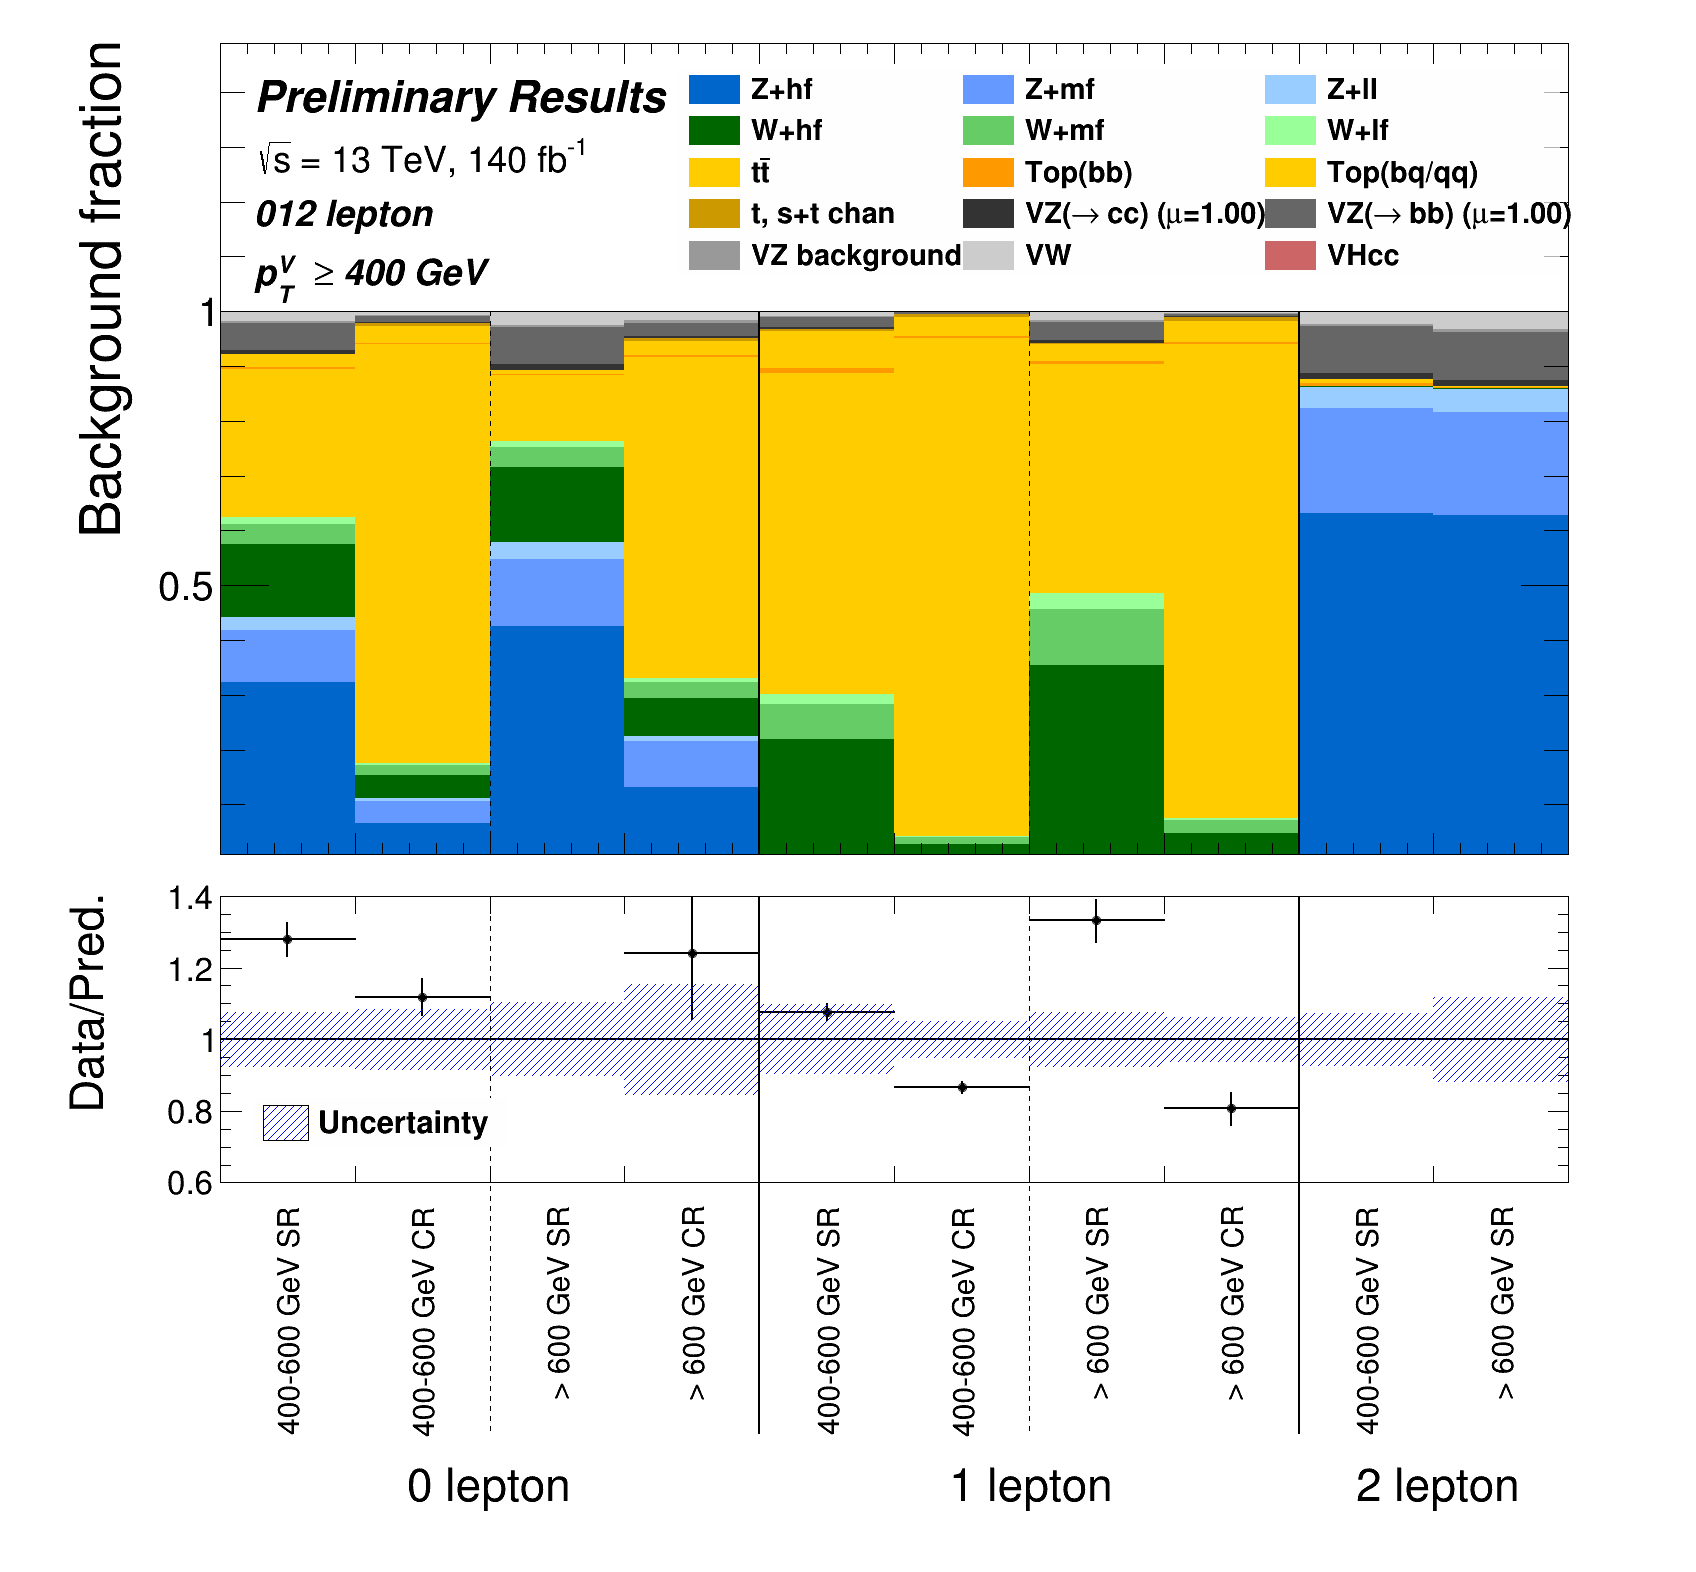
\includegraphics[width=\textwidth]{Images/VH/Own_fit/backCom_uncPrefit/GlobalFit_unconditional__Prefit/C_SRCRs_L012_BMin400.png}
            \caption{Boosted regime ($\geq 400$ GeV).}
            \label{fig:backCom_boos}
        \end{subfigure}
        \begin{subfigure}[b]{0.37\textwidth}
            \centering
            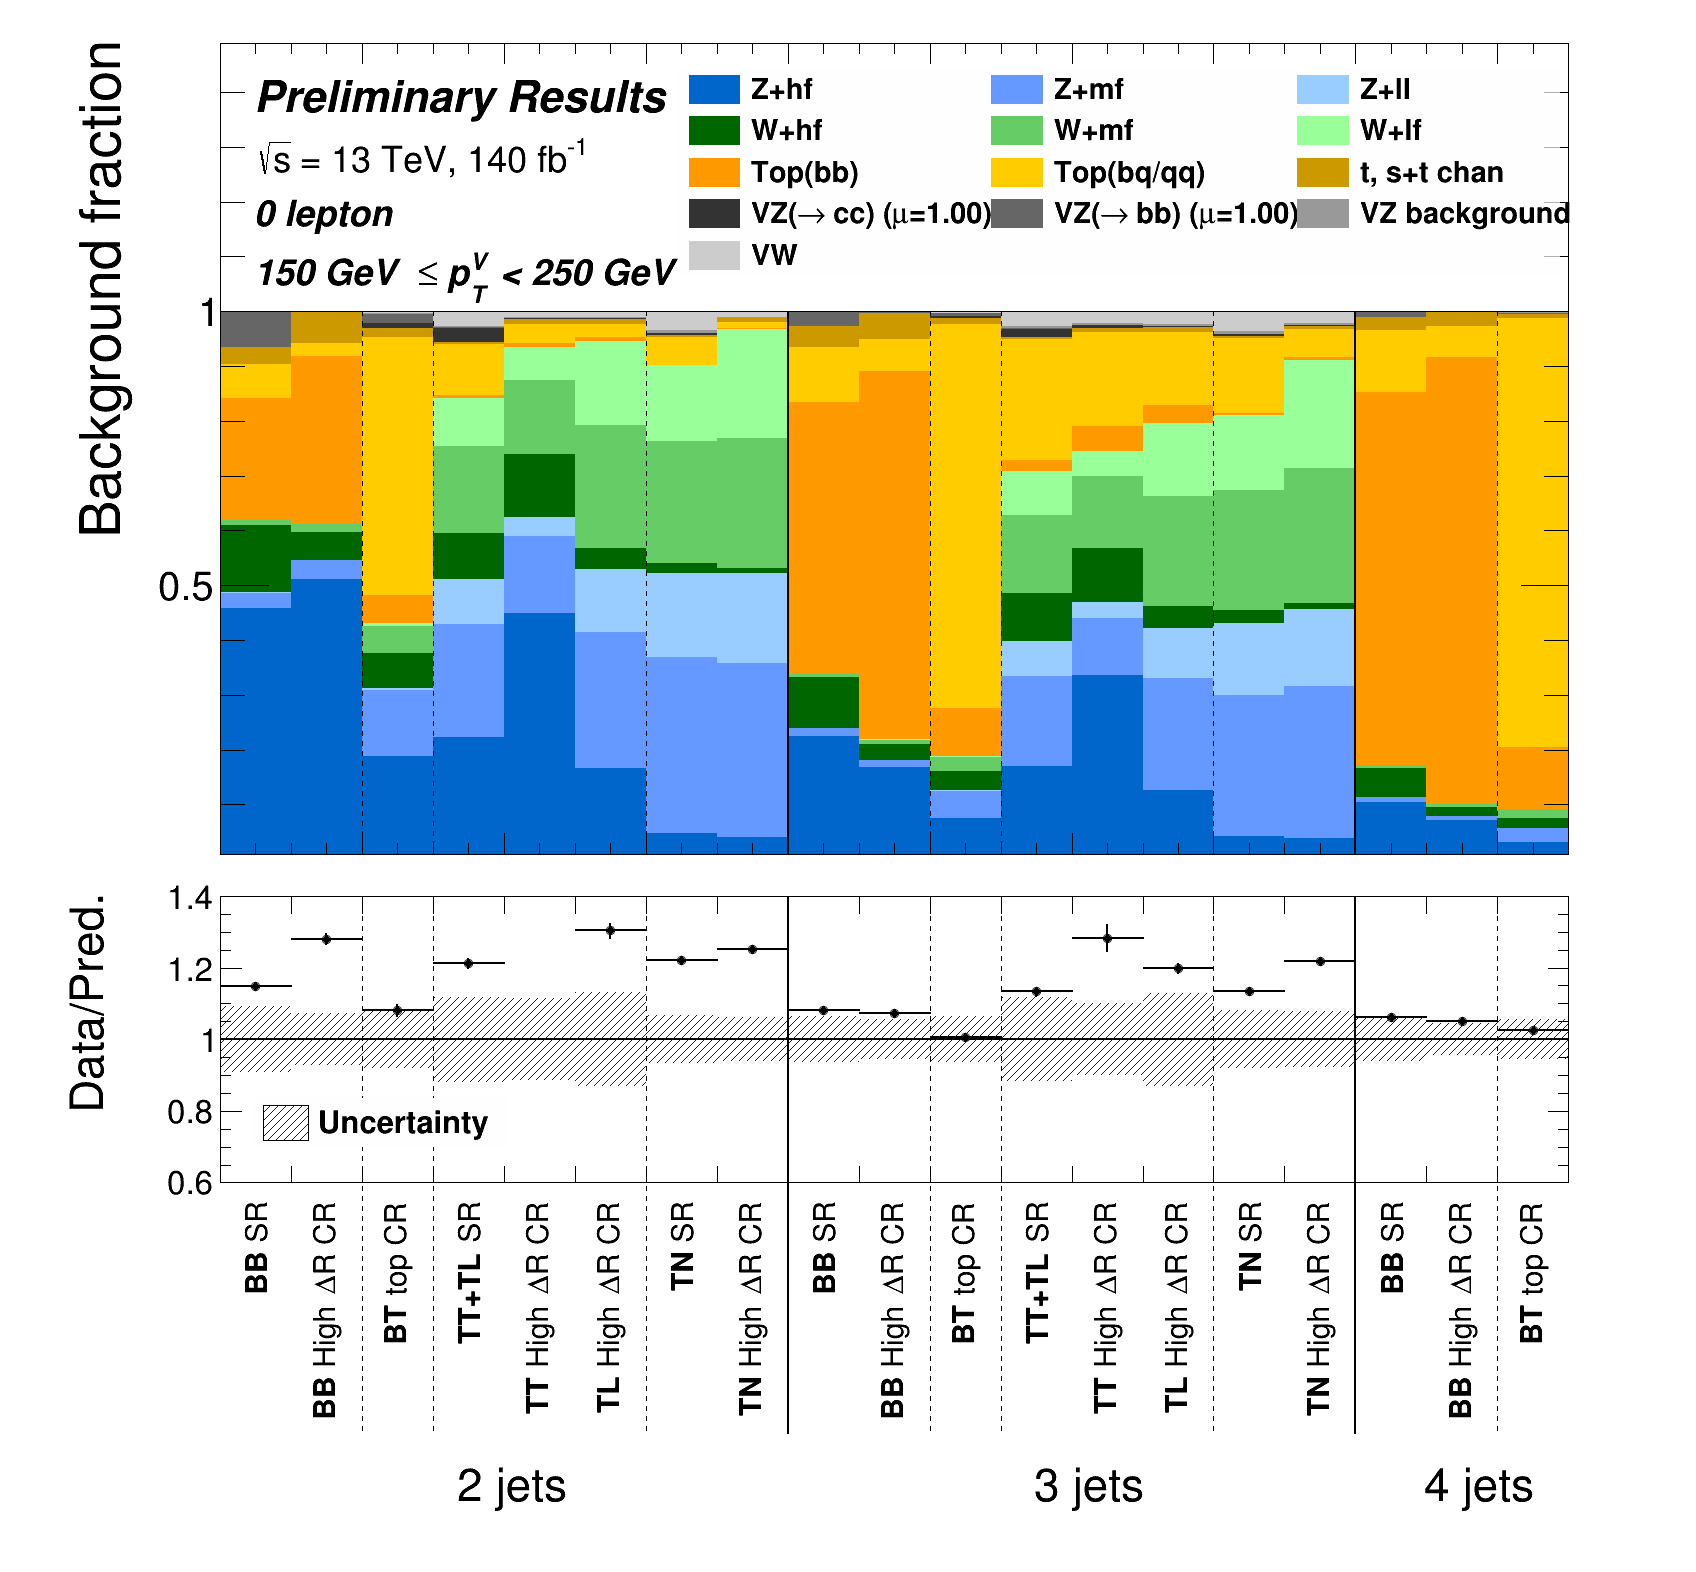
\includegraphics[width=\textwidth]{Images/VH/Own_fit/backCom_uncPrefit/GlobalFit_unconditional__Prefit/C_SRCRs_L0_BMax250_BMin150.png}
            \caption{0L, \ptv\ $\in$ [150, 250] GeV.}
            \label{fig:backCom_0L_1}
        \end{subfigure}
        \begin{subfigure}[b]{0.37\textwidth}
            \centering
            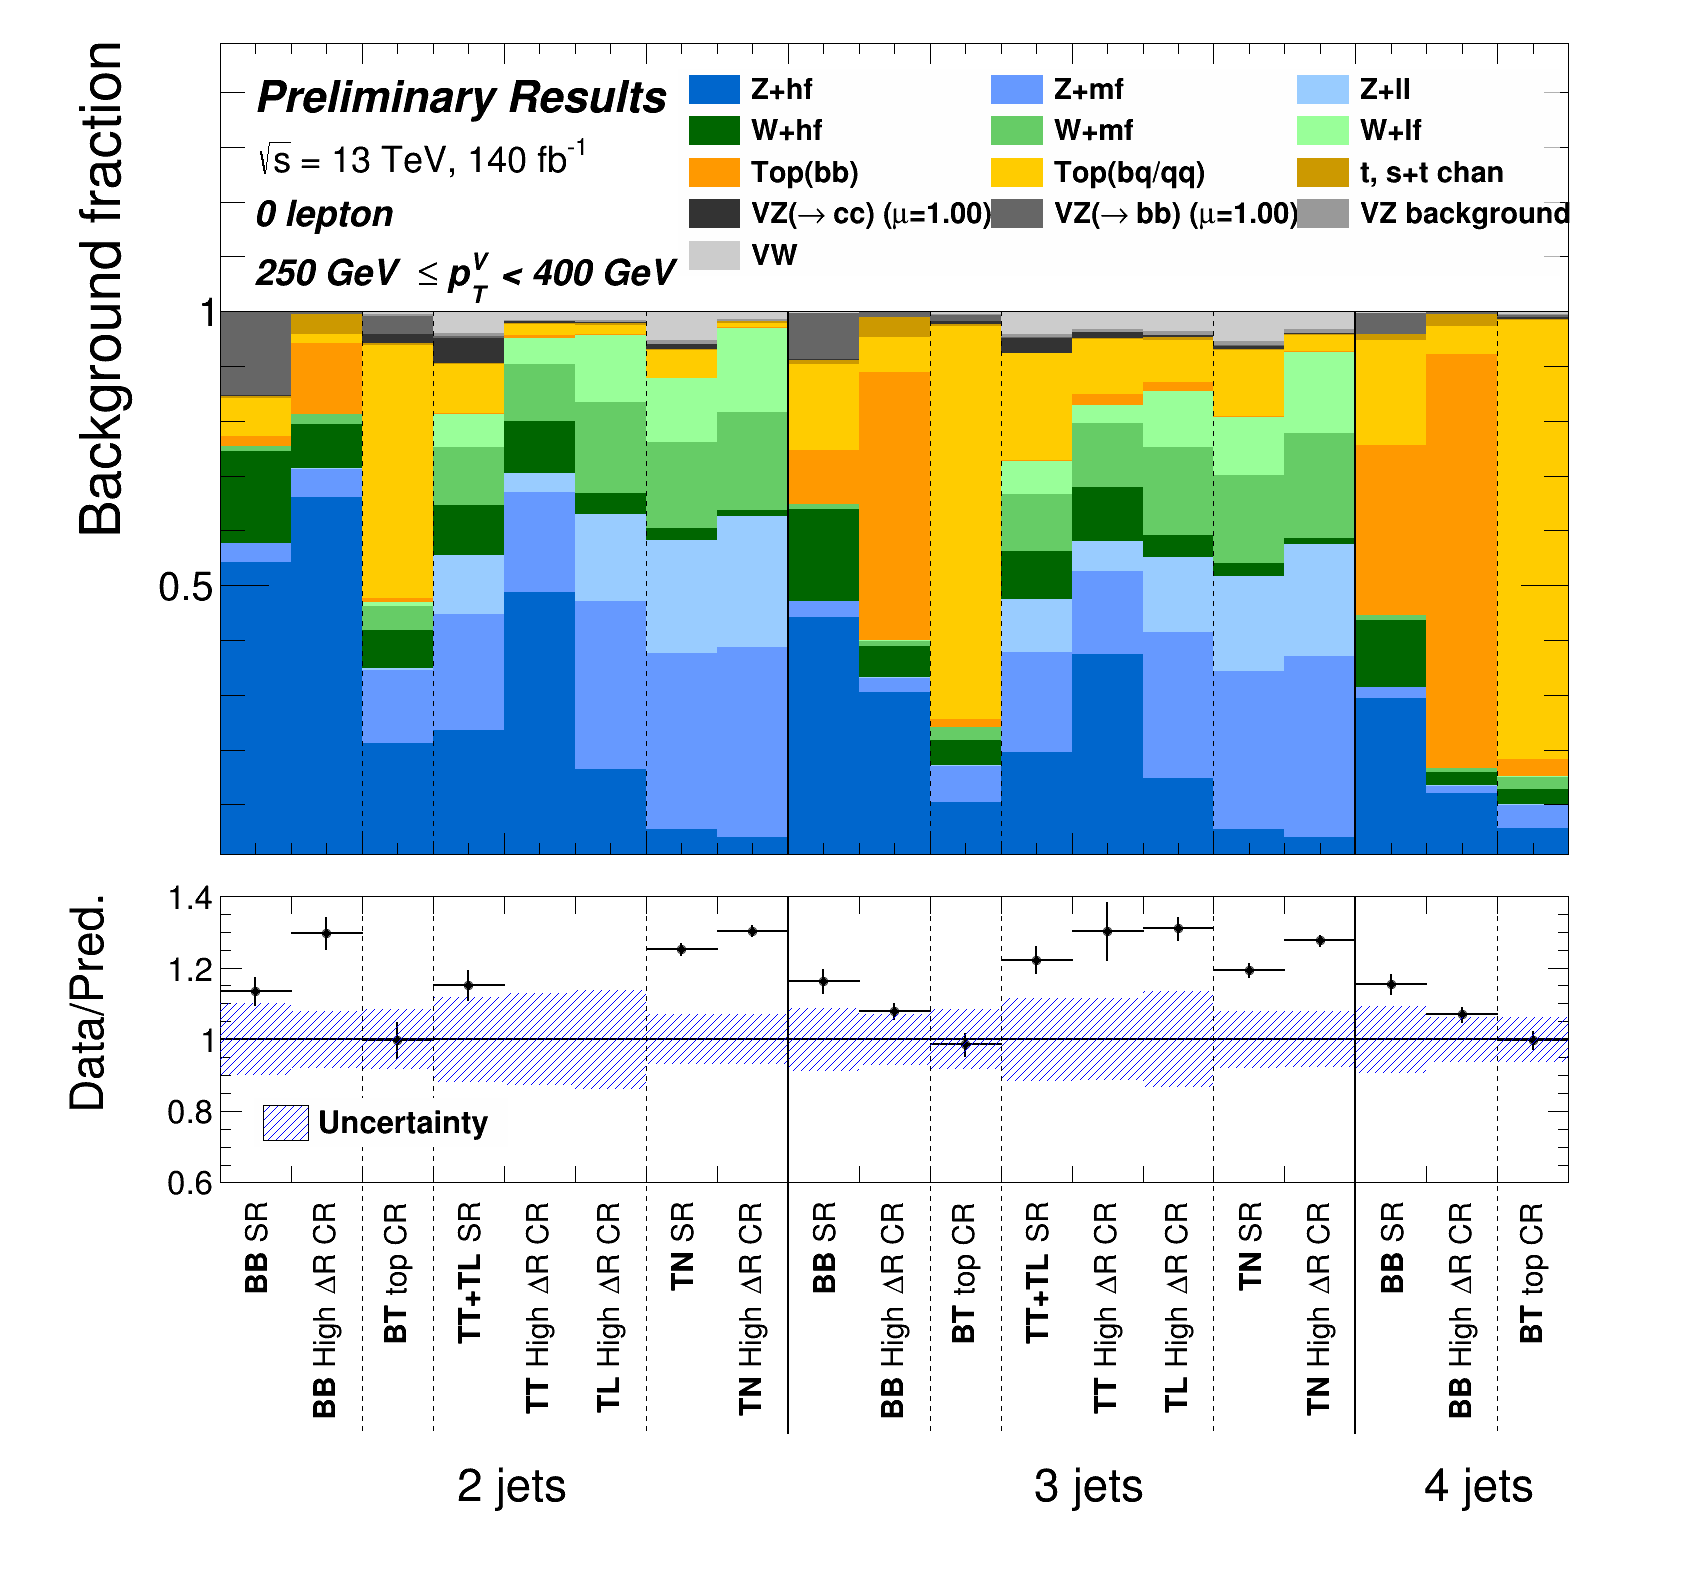
\includegraphics[width=\textwidth]{Images/VH/Own_fit/backCom_uncPrefit/GlobalFit_unconditional__Prefit/C_SRCRs_L0_BMax400_BMin250.png}
            \caption{0L, \ptv\ $\in$ [250, 400] GeV.}
            \label{fig:backCom_0L_2}
        \end{subfigure} 
    }\\
    %\hspace{-2cm}
    \makebox[\linewidth][c]{%
        \begin{subfigure}[b]{0.37\textwidth}
            \centering
            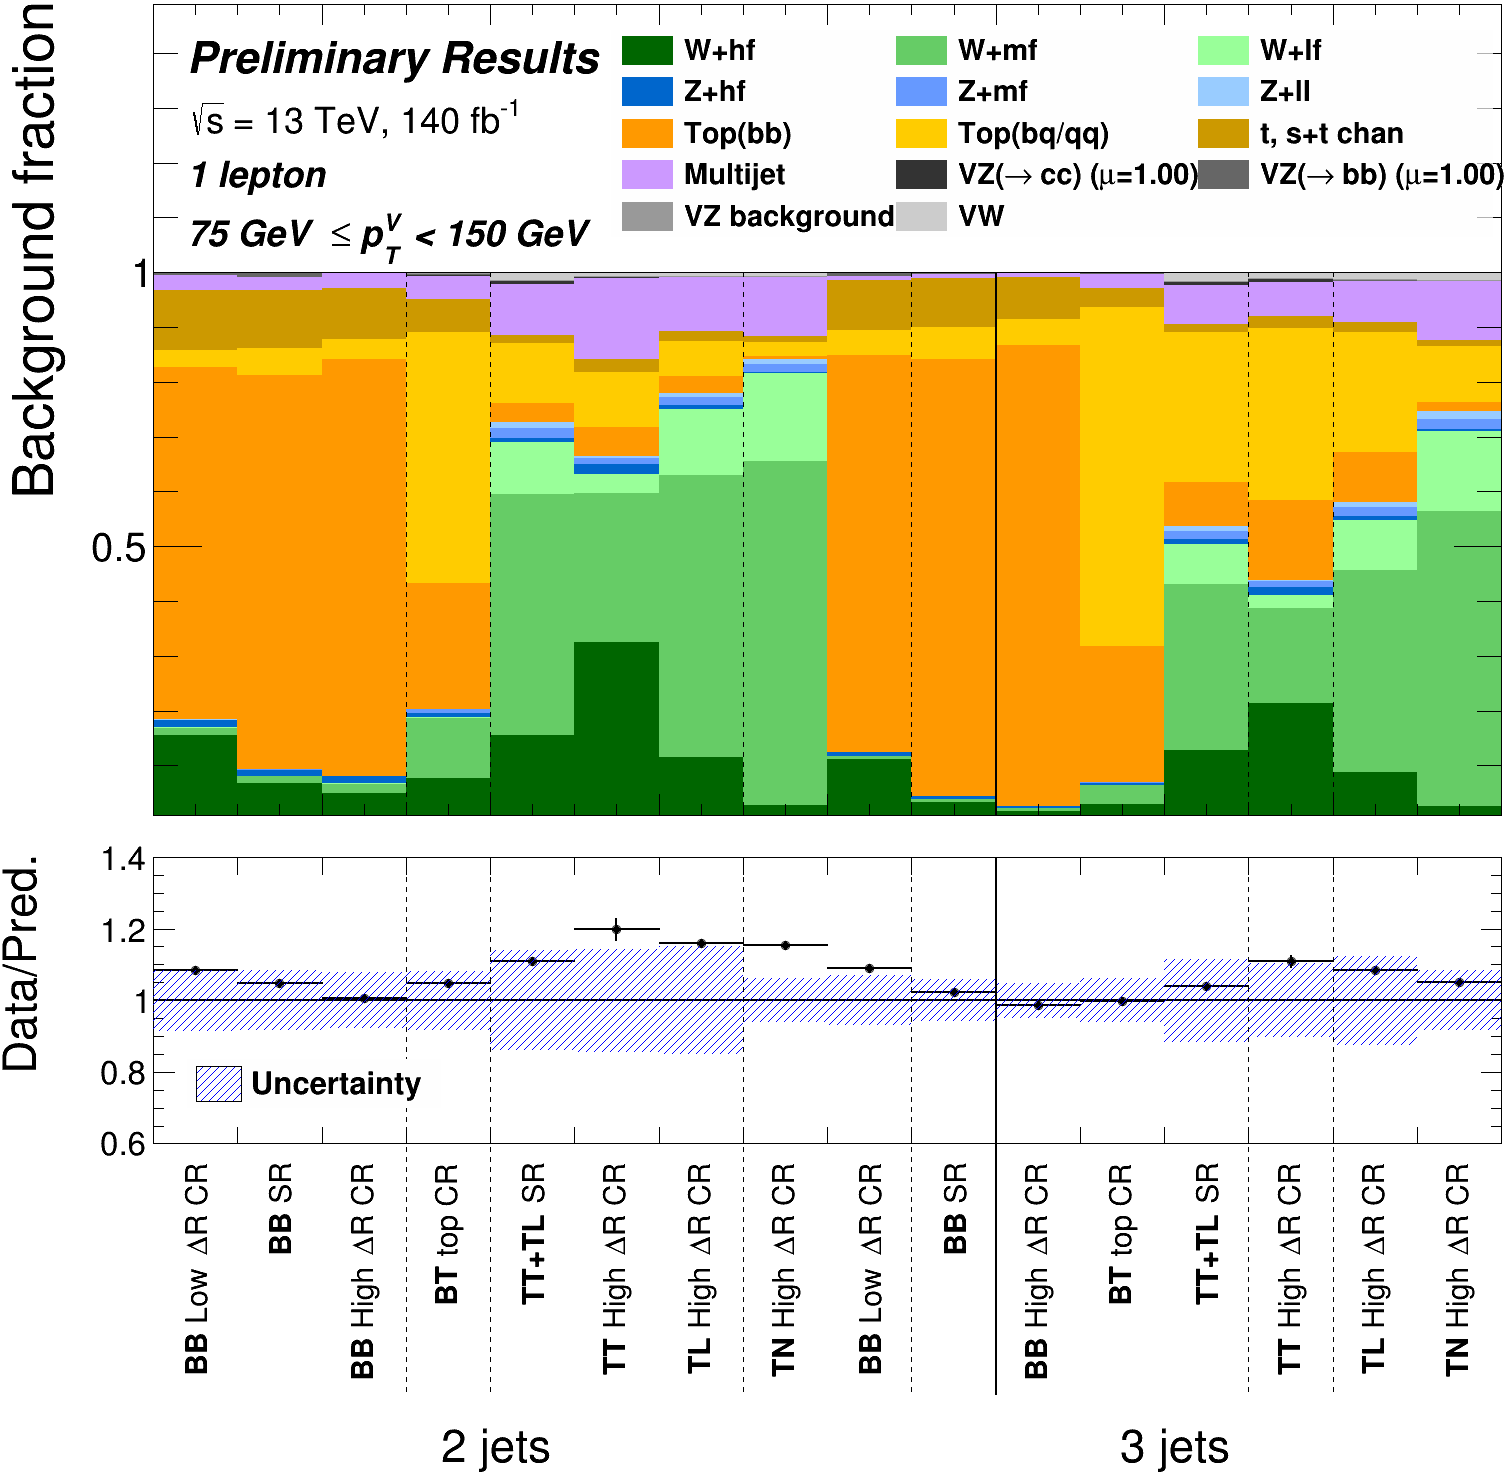
\includegraphics[width=\textwidth]{Images/VH/Own_fit/backCom_uncPrefit/GlobalFit_unconditional__Prefit/C_SRCRs_L1_BMax150_BMin75.png}
            \caption{1L, \ptv\ $\in$ [75, 150] GeV.}
            \label{fig:backCom_1L_1}
        \end{subfigure}
        \begin{subfigure}[b]{0.37\textwidth}
            \centering
            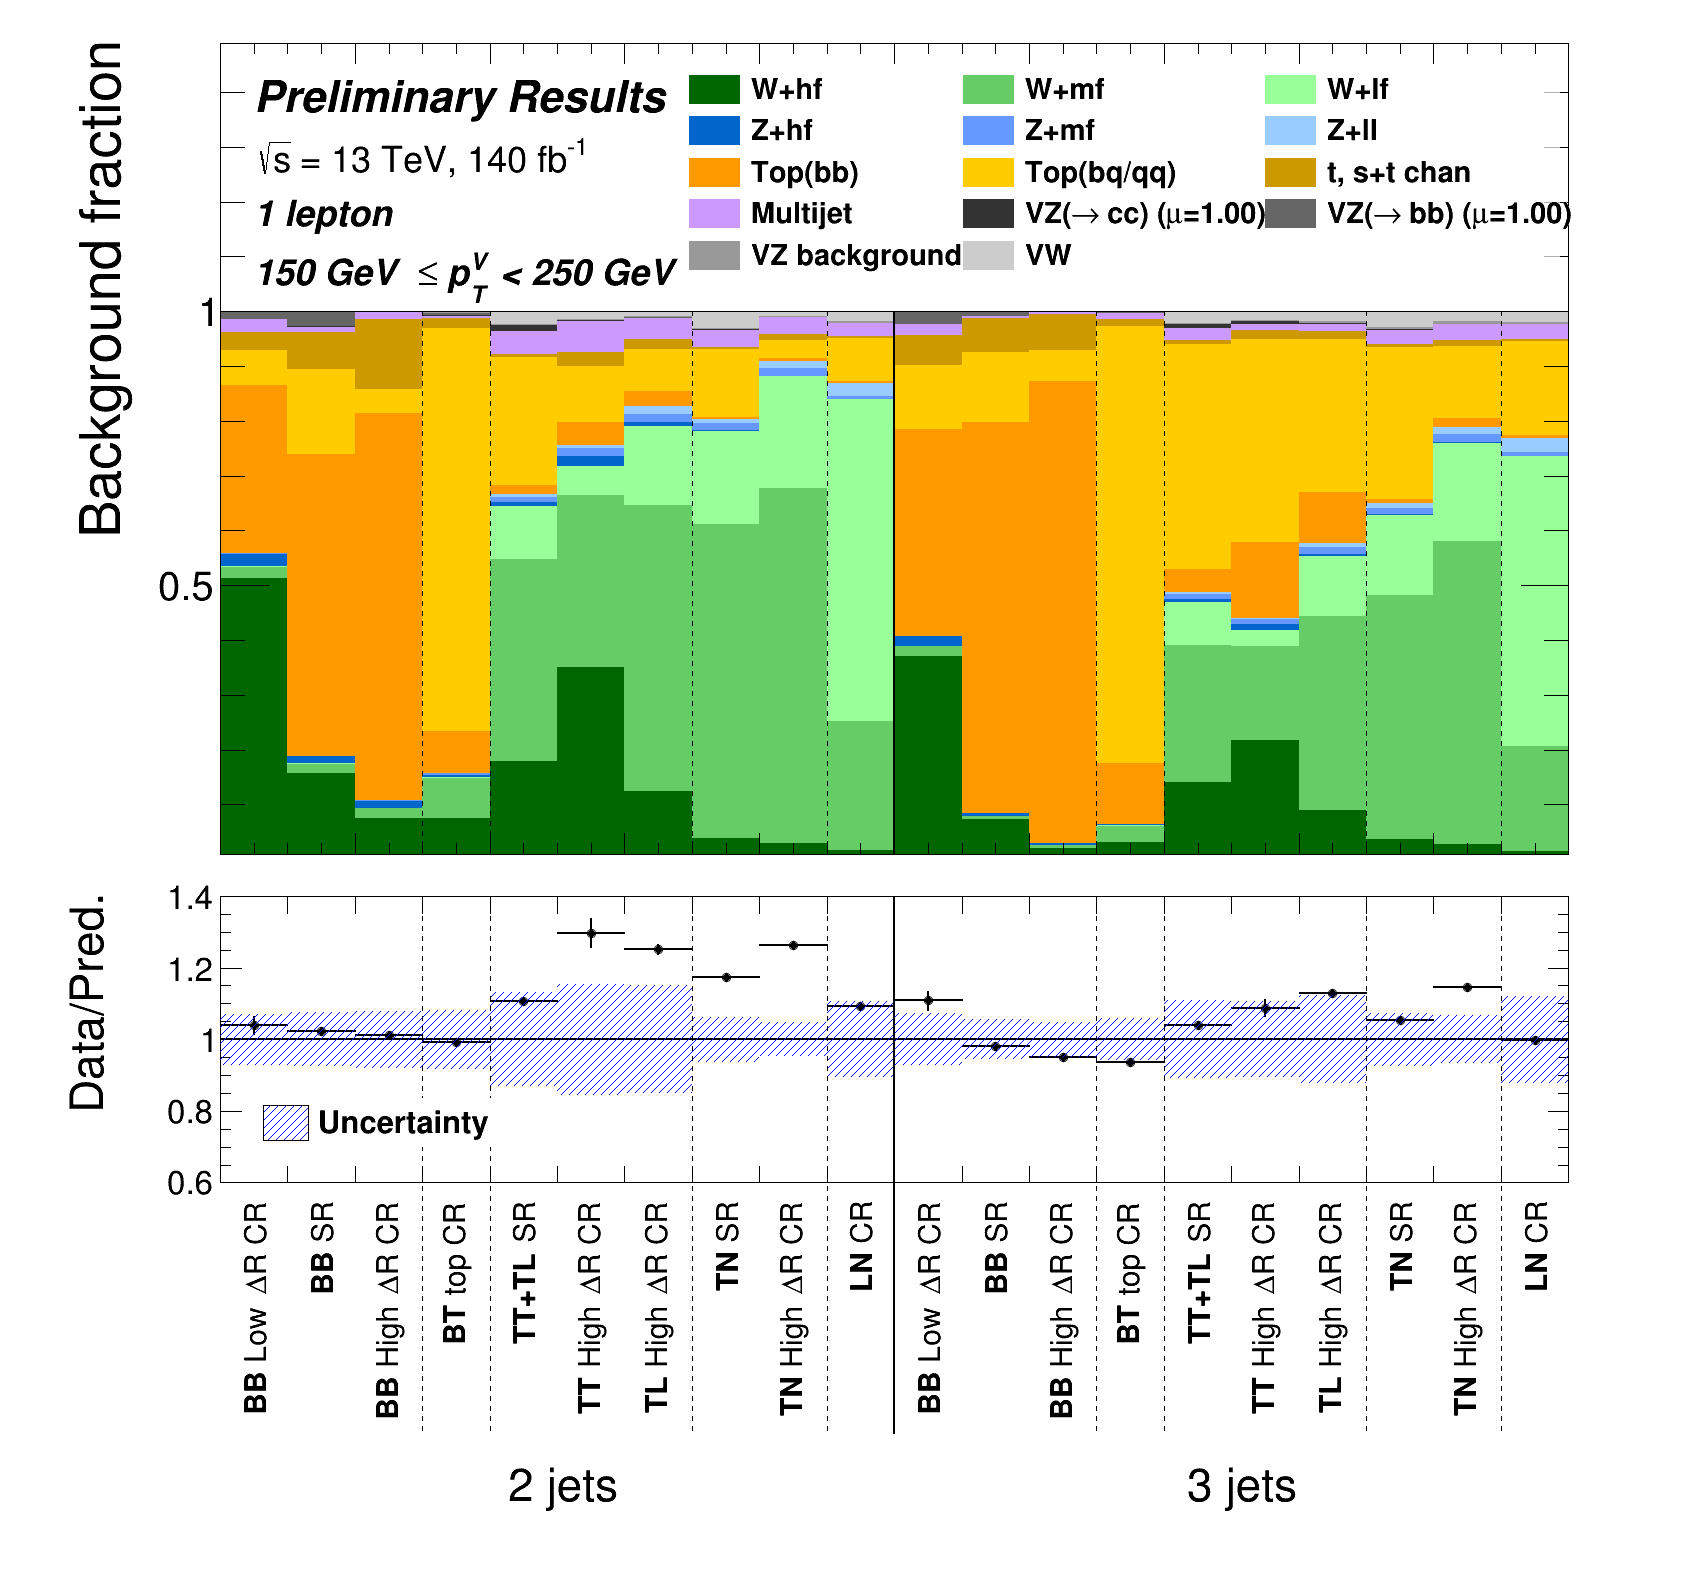
\includegraphics[width=\textwidth]{Images/VH/Own_fit/backCom_uncPrefit/GlobalFit_unconditional__Prefit/C_SRCRs_L1_BMax250_BMin150.png}
            \caption{1L, \ptv\ $\in$ [150, 250] GeV.}
            \label{fig:backCom_1L_2}
        \end{subfigure}
        \begin{subfigure}[b]{0.37\textwidth}
        \centering
        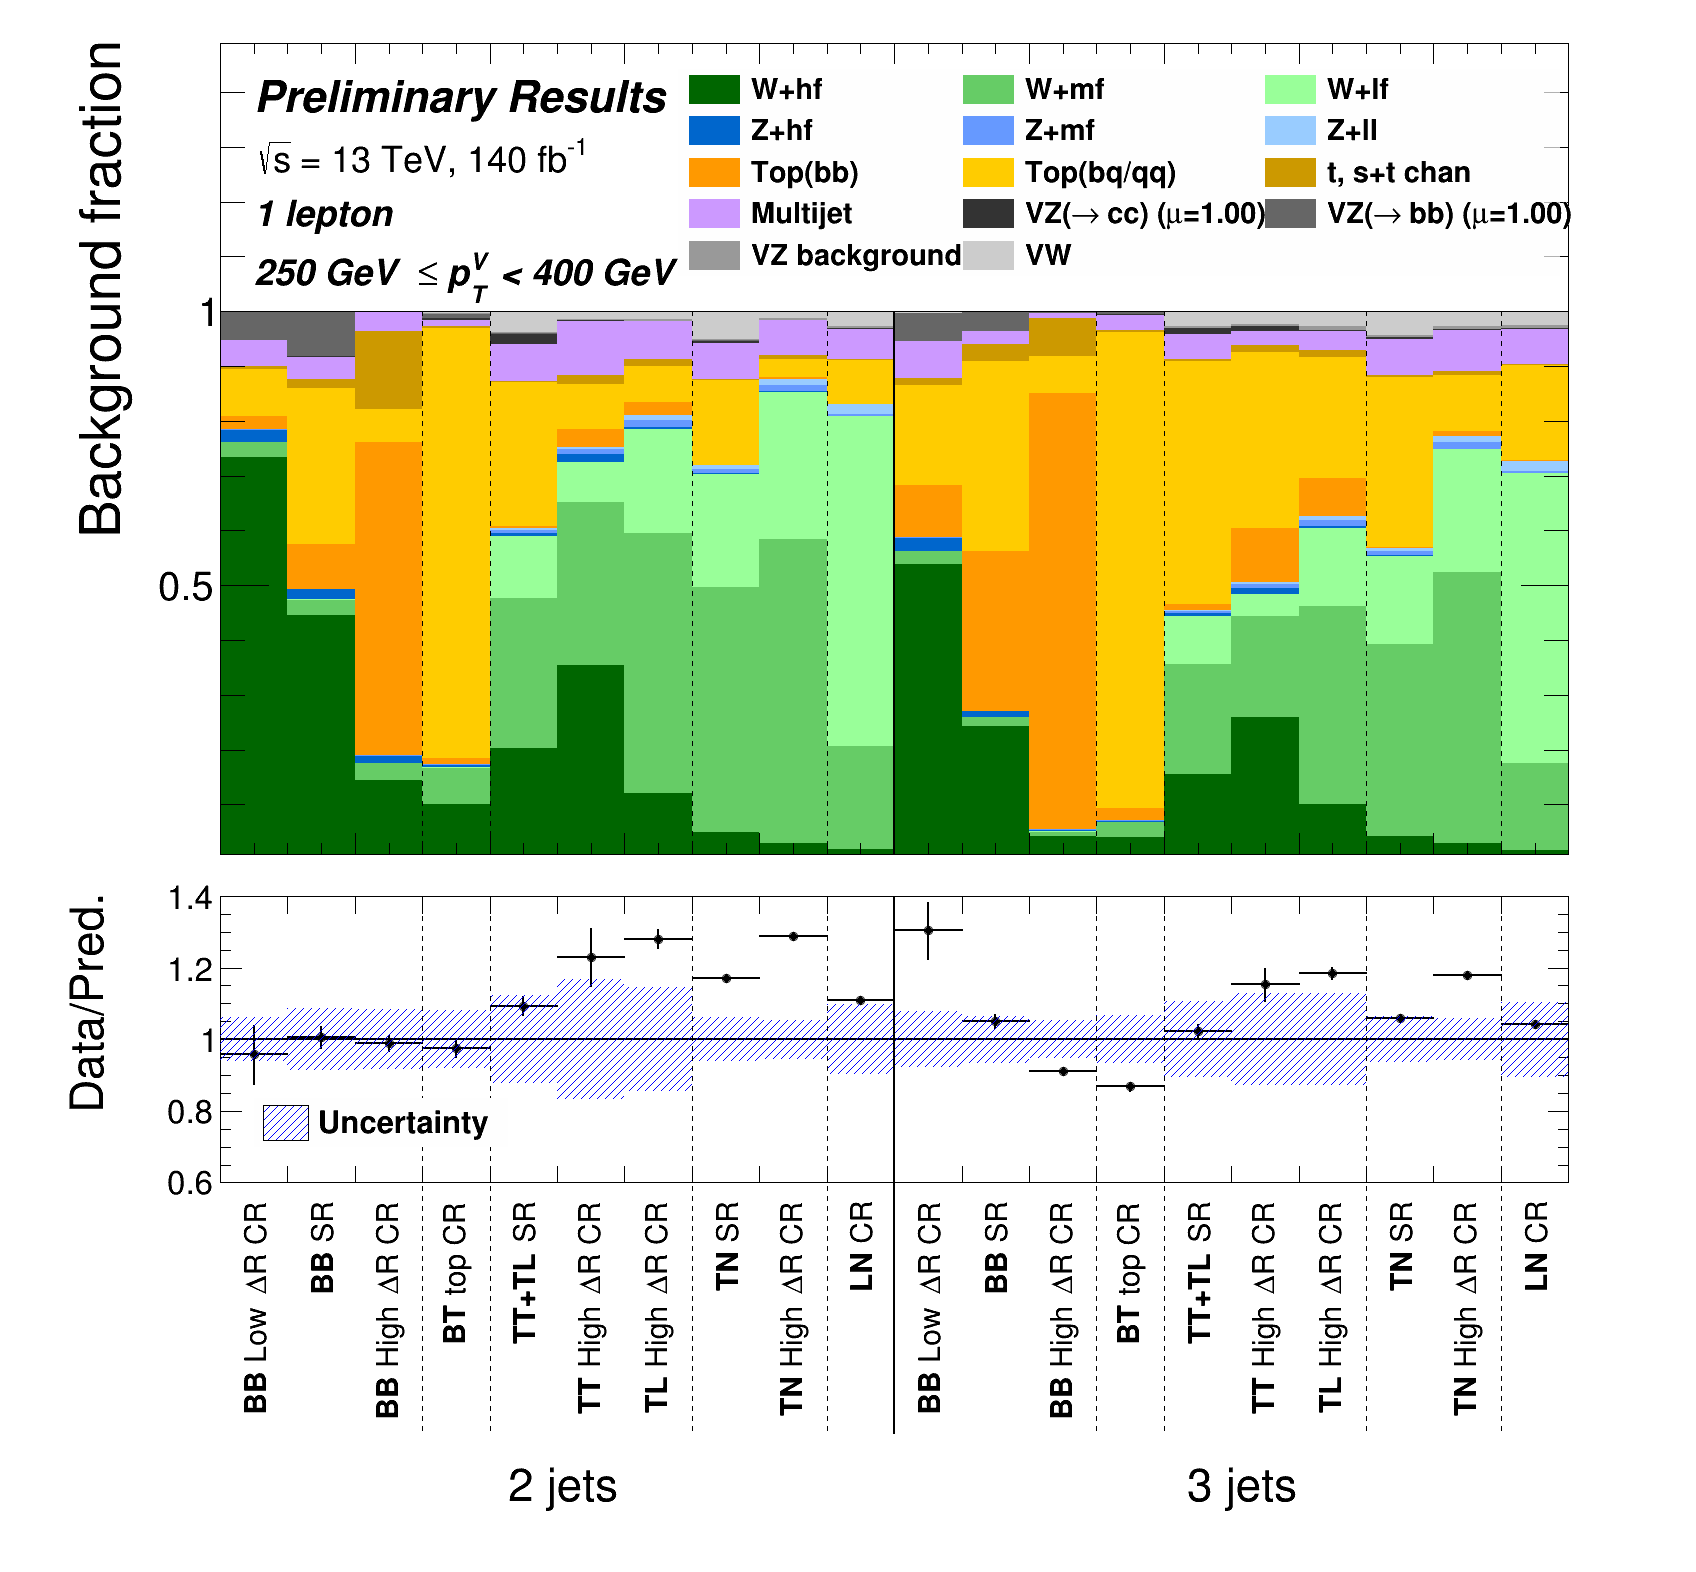
\includegraphics[width=\textwidth]{Images/VH/Own_fit/backCom_uncPrefit/GlobalFit_unconditional__Prefit/C_SRCRs_L1_BMax400_BMin250.png}
        \caption{1L, \ptv\ $\in$ [250, 400] GeV.}
        \label{fig:backCom_1L_3}
        \end{subfigure} 
    }   \\
    %\hspace{-2cm}
    \makebox[\linewidth][c]{%
        \begin{subfigure}[b]{0.37\textwidth}
            \centering
            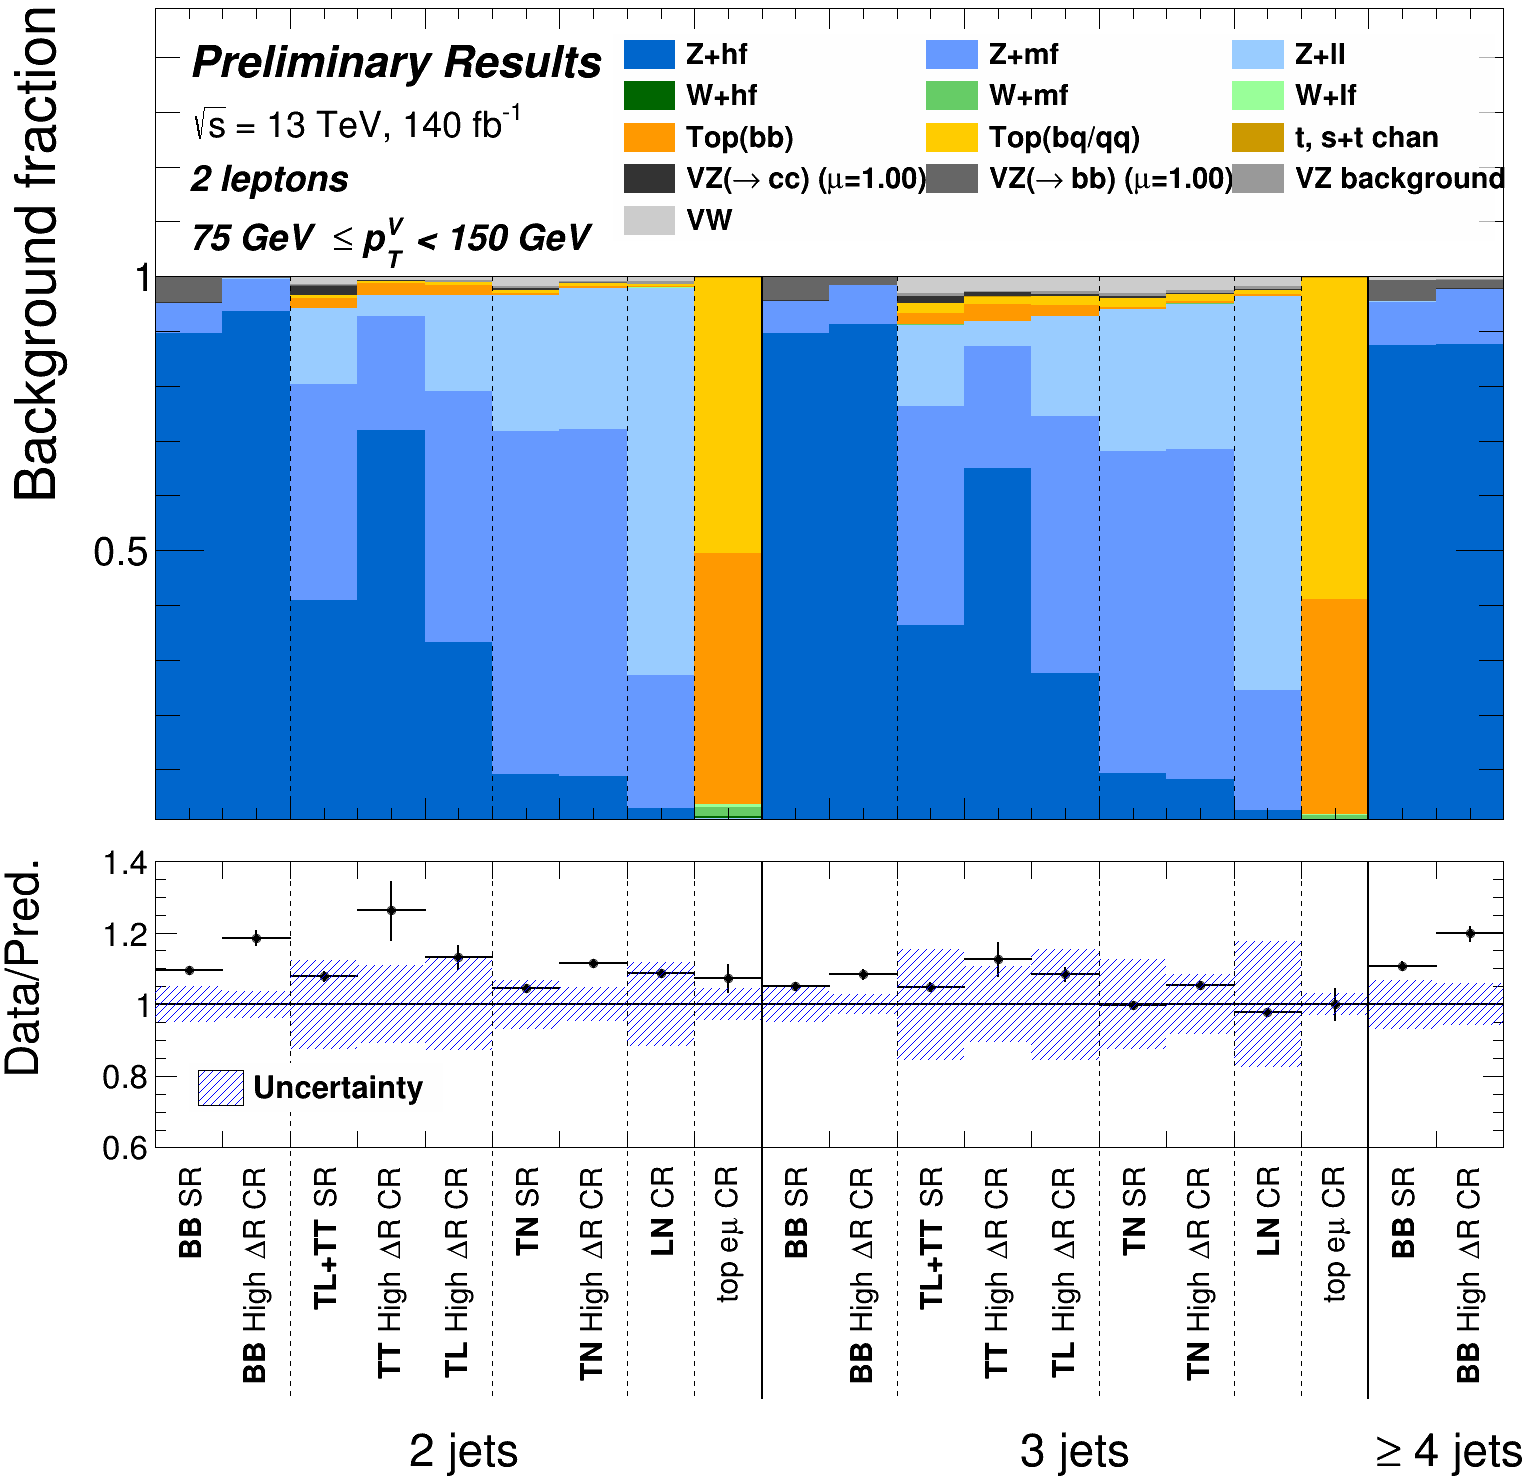
\includegraphics[width=\textwidth]{Images/VH/Own_fit/backCom_uncPrefit/GlobalFit_unconditional__Prefit/C_SRCRs_L2_BMax150_BMin75.png}
            \caption{2L, \ptv\ $\in$ [75, 150] GeV.}
            \label{fig:backCom_2L_1}
        \end{subfigure}
        \begin{subfigure}[b]{0.37\textwidth}
            \centering
            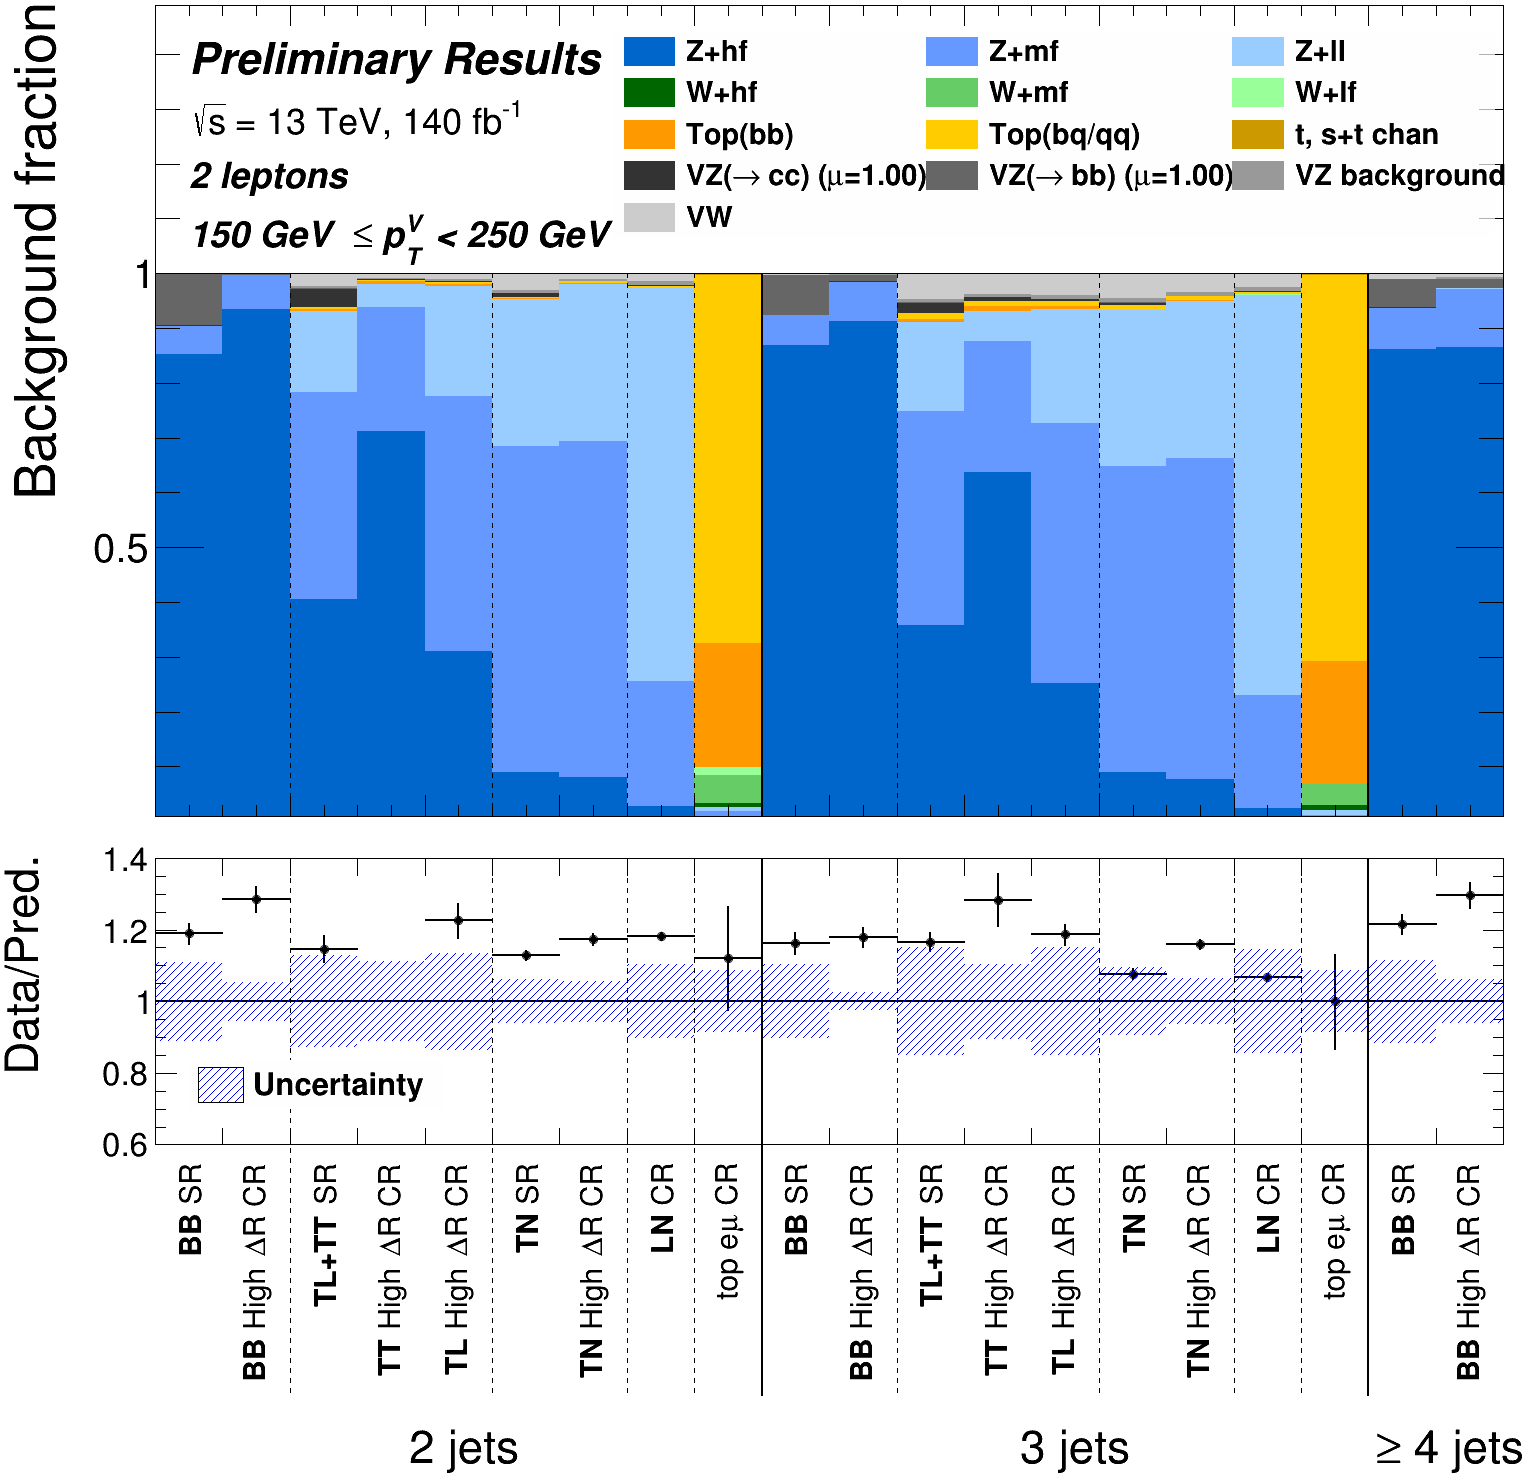
\includegraphics[width=\textwidth]{Images/VH/Own_fit/backCom_uncPrefit/GlobalFit_unconditional__Prefit/C_SRCRs_L2_BMax250_BMin150.png}
            \caption{2L, \ptv\ $\in$ [150, 250] GeV.}
            \label{fig:backCom_2L_2}
        \end{subfigure}
        \begin{subfigure}[b]{0.37\textwidth}
            \centering
            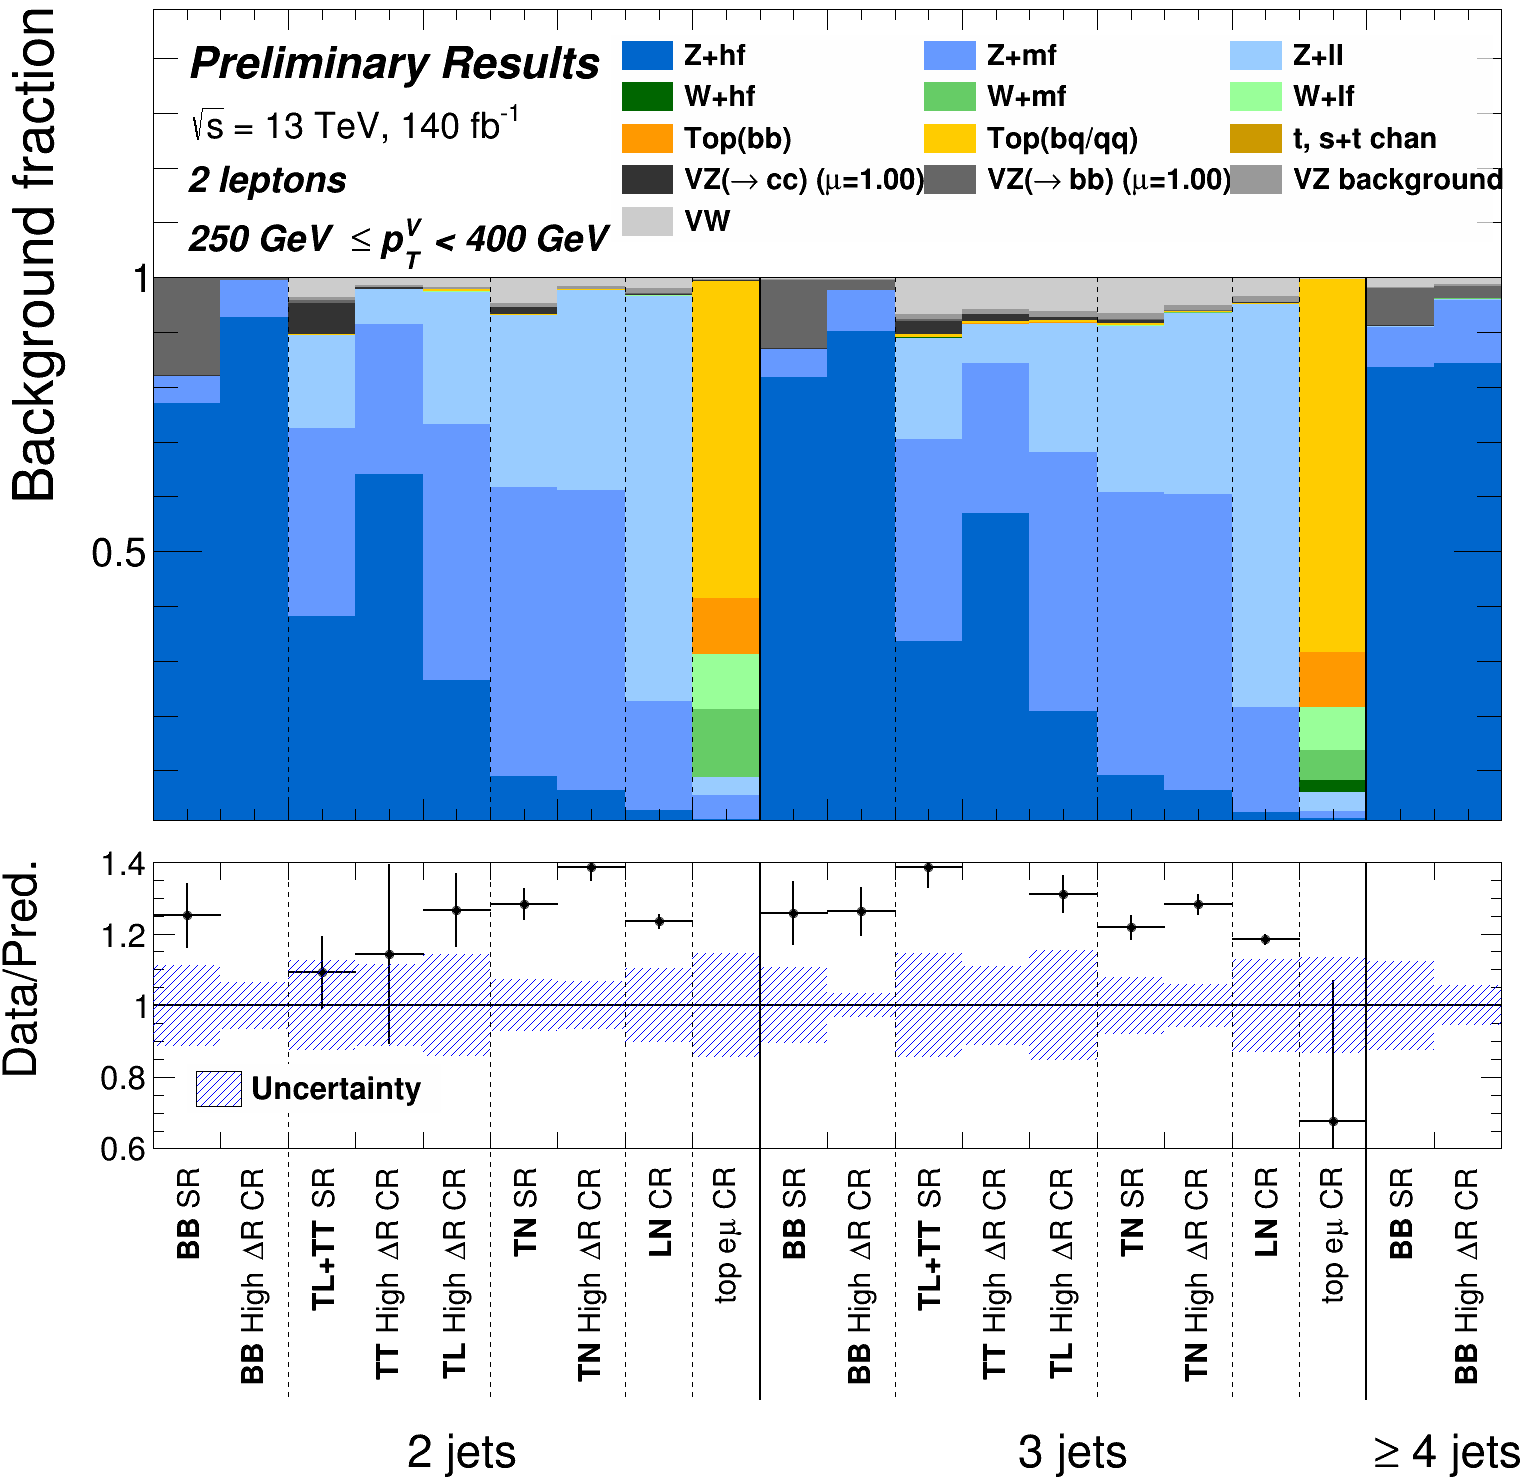
\includegraphics[width=\textwidth]{Images/VH/Own_fit/backCom_uncPrefit/GlobalFit_unconditional__Prefit/C_SRCRs_L2_BMax400_BMin250.png}
            \caption{2L, \ptv\ $\in$ [250, 400] GeV.}
            \label{fig:backCom_2L_3}
        \end{subfigure} 
    }
    \caption{The background composition of the different analysis regimes and lepton channels, with the data - Monte Carlo prefit agreement displayed in the bottom panels.}
    \label{fig:backCom}
\end{figure} 

\section{Signals \& Backgrounds Modelling}\label{sec-mod}
Similarly to the experimental process, the simulations of the signals and backgrounds cannot entirely be accurate and mis-modellings are to be expected in the derived samples. These inaccuracies must be taken into account in the fit to avoid introducing bias. The modelling of the signals and backgrounds in the \vhbc\ combined analysis is discussed in this section. The composition of the different processes changes depending on the lepton channel and the analysis category, as shown in Figure \ref{fig:backCom}. The $V$+jets backgrounds are the dominant ones in the signal regions of the 0-lepton and 2-lepton channels, while the top processes contribute more in the 1-lepton channel, and globally at larger jet multiplicities and lower \ptv. Due to flavour tagging, \vhb\ primarily selects the $bb$-component of the background while \vhc\ has more diverse flavour compositions with the 2 $c$-tag as an intermediate step between the $BB$ and 1 $c$-tag. This translates into increased \vhf\ fractions in \vhb\ and \vmf\ and \vlf\ in \vhc. In summary:
\begin{itemize}
    \item \textbf{0-lepton}: the dominant background is the $Z$+jets with a sizeable $W+$jets component, particularly in \vhc\ due to large \etm\ or a miss-identified hadronic $\tau$ and some top backgrounds for the \vhb\ side particularly. In \vhb\ there is a significant top-background contribution, with this process dominating in 3- and 4-jets. In addition, this lepton channel has some diboson contribution.
    \item \textbf{1-lepton}: the top process is dominant for \vhb, while for \vhc\ a sizeable $W+$jets leads followed by the top. There is also a visible multi-jet contribution.  
    \item \textbf{2-lepton}: most of the background is made of $Z+$jets, followed by the diboson and some residual top process at low \ptv\ for \vhb. 
\end{itemize}
The different background contributions to each analysis region require an adequate strategy to constrain their modelling in the fit, as detailed in this section.
  
\subsection{General Modelling Strategy}\label{sec-modStrat}
The combined analysis adopts some common strategies to model the backgrounds and signals that are described in this section before reviewing the specificities adopted for each process. A guideline for the modelling is to treat backgrounds coherently across analysis regimes and correlate uncertainties between the \vhb\ and \vhc\ sides when possible. The normalisations of the major backgrounds, the $V+$jets and Top, are free to float in the fit, with \gls{fn} split by \ptv\ and jet multiplicity when the statistics allow. Minor backgrounds are fixed at \gls{mc} predictions with a normalisation uncertainty. To account for \gls{mc}-generator modelling uncertainty, comparisons of the nominal samples to alternative samples introduced in section \ref{sec-datasets} and summarised in Table \ref{tab:summary_altsamples} are performed. For each process, the uncertainties are split into normalisation, relative acceptance, and shape uncertainties.  % Check top s is treated like that;

\begin{table}[!h]
    \centering
    \begin{tabular}{llll}
      \hline \hline 
      \textbf{Sample} & \textbf{Nominal Generator} & \textbf{Alternative Generators} & \textbf{Systematics Effects} \\
      \hline
      \vhb\ & \textsc{Powheg} + \textsc{Pythia 8} & \textsc{Powheg} + \textsc{Herwig 7} & $\mu_R$, $\mu_F$, \gls{isr}, \gls{fsr}, \gls{pdf}\\
      \hline
      \vhc\ & \textsc{Powheg} + \textsc{Pythia 8} & \textsc{Powheg} + \textsc{Herwig 7} & $\mu_R$, $\mu_F$, \gls{isr}, \gls{fsr}, \gls{pdf} \\
      \hline
      $V$+jets & \textsc{Sherpa} 2.2.11 & \textsc{MadGraph5 FxFx}, & $\mu_R$, $\mu_F$, \gls{pdf}, \\
                                            & & \textsc{Sherpa} 2.2.1 & EW corrections \\
      \hline
      \ttb\ \& & \textsc{Powheg}+\textsc{Pythia} 8 & \textsc{Powheg}+\textsc{Herwig} 7,  & \gls{isr}, \gls{fsr}, \\
      single-top &  & \textsc{MadGraph5}+\textsc{Pythia} 8  & DS/DR (single-top $Wt$) \\
      \hline
      Diboson & \textsc{Sherpa} 2.2.11  & \textsc{Powheg}+\textsc{Pythia} 8, & $\mu_R$, $\mu_F, \gls{pdf}$,\\
       &  & \textsc{Sherpa} 2.2.1 & EW corrections\\
      \hline \hline 
    \end{tabular}
    \caption{Summary of nominal and alternative samples in the analysis. Alternative samples include different generator and systematics effects from modification to the nominal setup.}
    \label{tab:summary_altsamples}
\end{table}
  
\paragraph{Normalisation uncertainties} are an overall uncertainty on the yield of a process, computed in and applied to all regions. These uncertainties are applied when the yield of a background to derive its normalisation from data, e.g., for the diboson and single-top $s$ processes.

\paragraph{Acceptance uncertainties:} relative acceptance uncertainties for each process cover possible changes in the distribution of events of the specific process across the different regions of the analysis phase space. They account for the migration of events between these regions and are assessed by measuring the change in the ratio of events between regions when switching to differently generated samples (indexed by $i$ here). The priors on these uncertainties are calculated with the double ratio of Equation \ref{eq-doubleRatio}:
\begin{equation}\label{eq-doubleRatio}
    \text{Acceptance Unc}_i = \frac{\text{Acceptance}[\text{Cat.}^B (\mathrm{alternative}_i\mathrm{\,\,MC})]}{\text{Acceptance}[\text{Cat.}^A (\mathrm{alternative}_i\mathrm{\,\,MC})]} \Bigg/ \frac{\text{Acceptance}[\text{Cat.}^B (\mathrm{nominal\,\,MC})]}{\text{Acceptance}[\text{Cat.}^A (\mathrm{nominal\,\,MC})]},
\end{equation}
where category $A$ ($\text{Cat.}^A$) is the region with the highest purity in the studied process, and $B$ ($\text{Cat.}^B$) is the region extrapolated to. If several alternative generators are used ($i > 1$), their respective double ratios are summed in quadrature: \[ \text{Total Acceptance Unc} = \sqrt{\sum_i\left(\text{Acceptance Unc}_i\right)^2}.\] If the extrapolation is across several regions $A$, $B$, $C$ ordered by decreasing purity, the acceptance ratio is decomposed into two extrapolations: a first one from $A \rightarrow B+C$ with an additional $B \rightarrow C$ uncertainty. Due to their similar kinematic definition, for acceptance uncertainties between distinct analysis regions in the resolved regime, the signal and Top $BT$ control regions are considered jointly. The acceptance uncertainties between these two regions are modelled by the flavour tagging uncertainties.

\paragraph{Shape uncertainties:} the \glspl{bdt}, $m_{bb}$, $m_{cc}$, and \ptv\ shapes of the processes in the different regions are given some flexibility in the fit by introducing shape uncertainties derived from a comparison of the nominal to the alternative samples. The combined analysis introduces the novel \gls{carl} technique to derive a reweighted shape uncertainty using a neural network \cite{carl}. A \gls{dnn} is trained to discriminate nominal events from alternative ones, with the process repeated for each alternative sample. The output of the \gls{carl} network is a score representing the probability for an event to belong to the alternative sample. This is used to reweight the nominal distribution into the alternative distribution, similarly to the process of truth tagging. The advantage of this technique is that the reweighted nominal distributions benefit from much larger statistics than the alternative ones, thus smoothing out bin fluctuations and reducing the \gls{mc} statistics uncertainties. Examples of such derived \gls{carl} shape uncertainties modelling the \gls{ps} with \textsc{MadGraph5\_aMC@NLO} for the single-top $Wt$ process in 1-lepton are presented in Figure \ref{fig:carl:resolved_closure_stopWt}. Additional shape uncertainties from \gls{ew} corrections, \gls{qcd} scales, $V+$jets and diboson \ptv\ modelling with \textsc{Sherpa} 2.2.1, parton shower alternative for the signal samples, and uncertainties for the single-top $Wt$ DS / DR shapes are directly derived by comparing samples.

\begin{figure}[!htbp]
    \centering
      \subfloat[SR BDT distribution.]{
        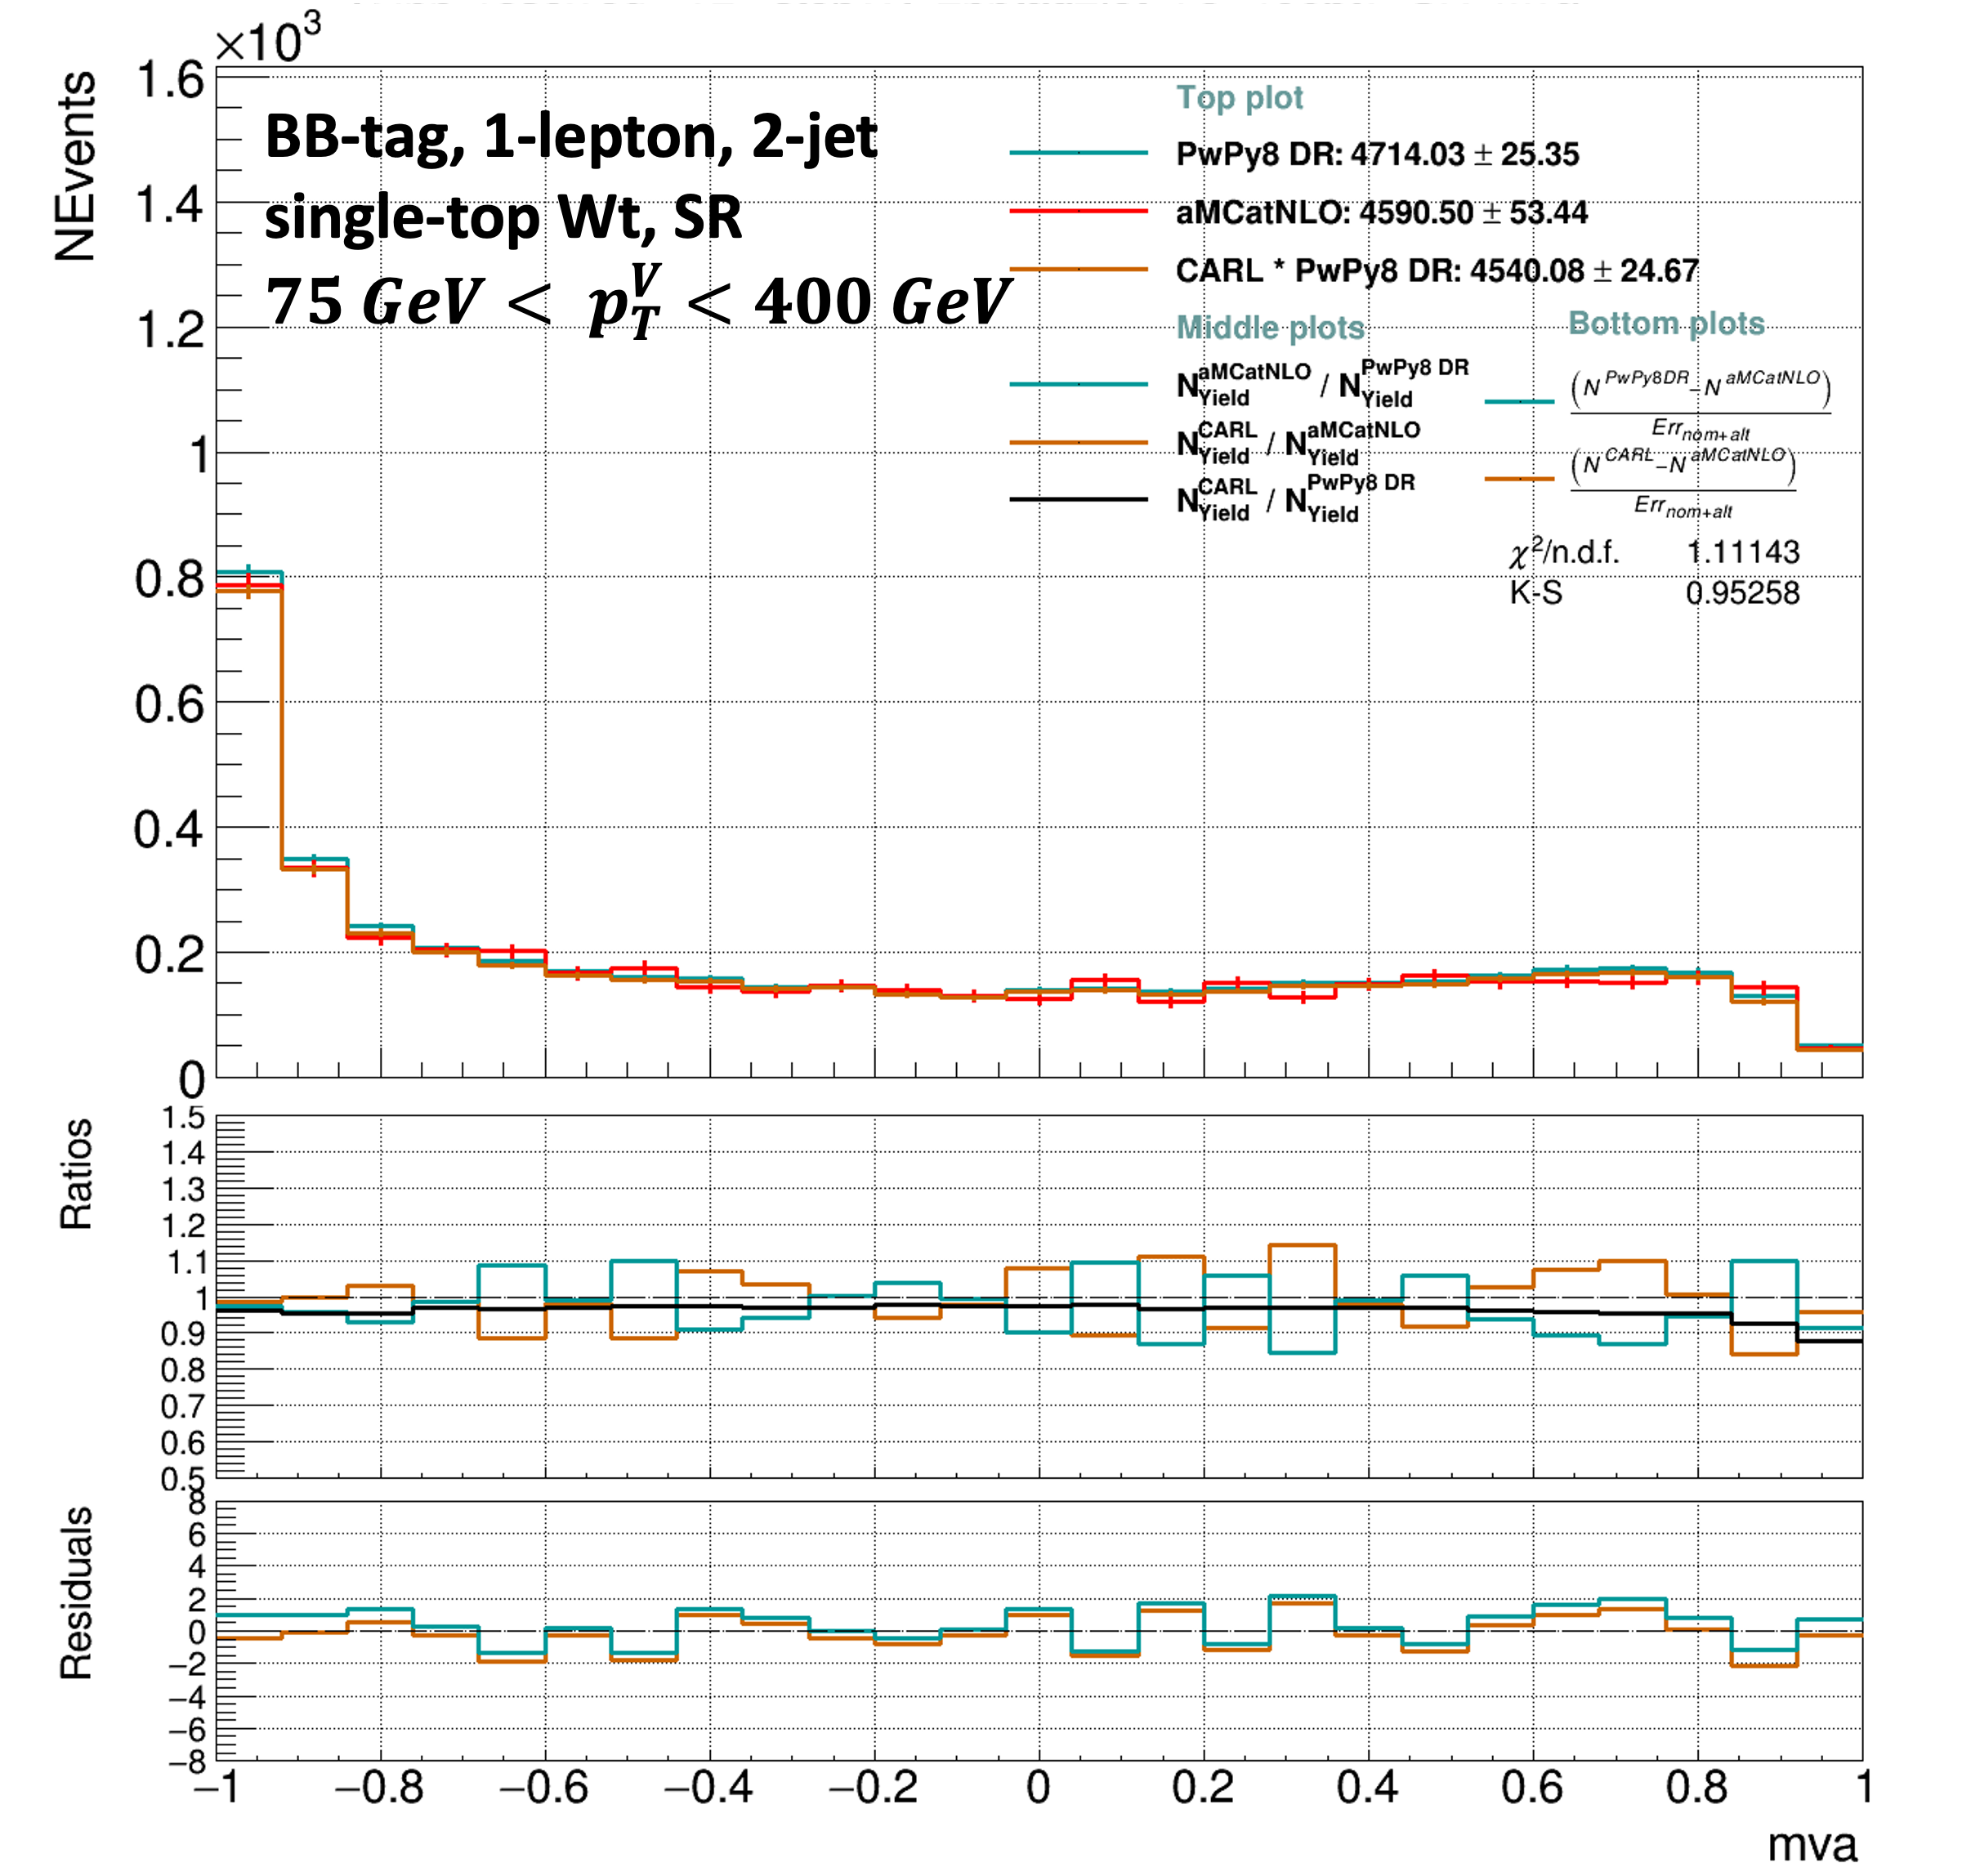
\includegraphics[width=0.48\textwidth]{Images/VH/Carl/wt/sr.png}
      }
      \subfloat[\highdr\ CR $m_{bb}$ distribution.]{
        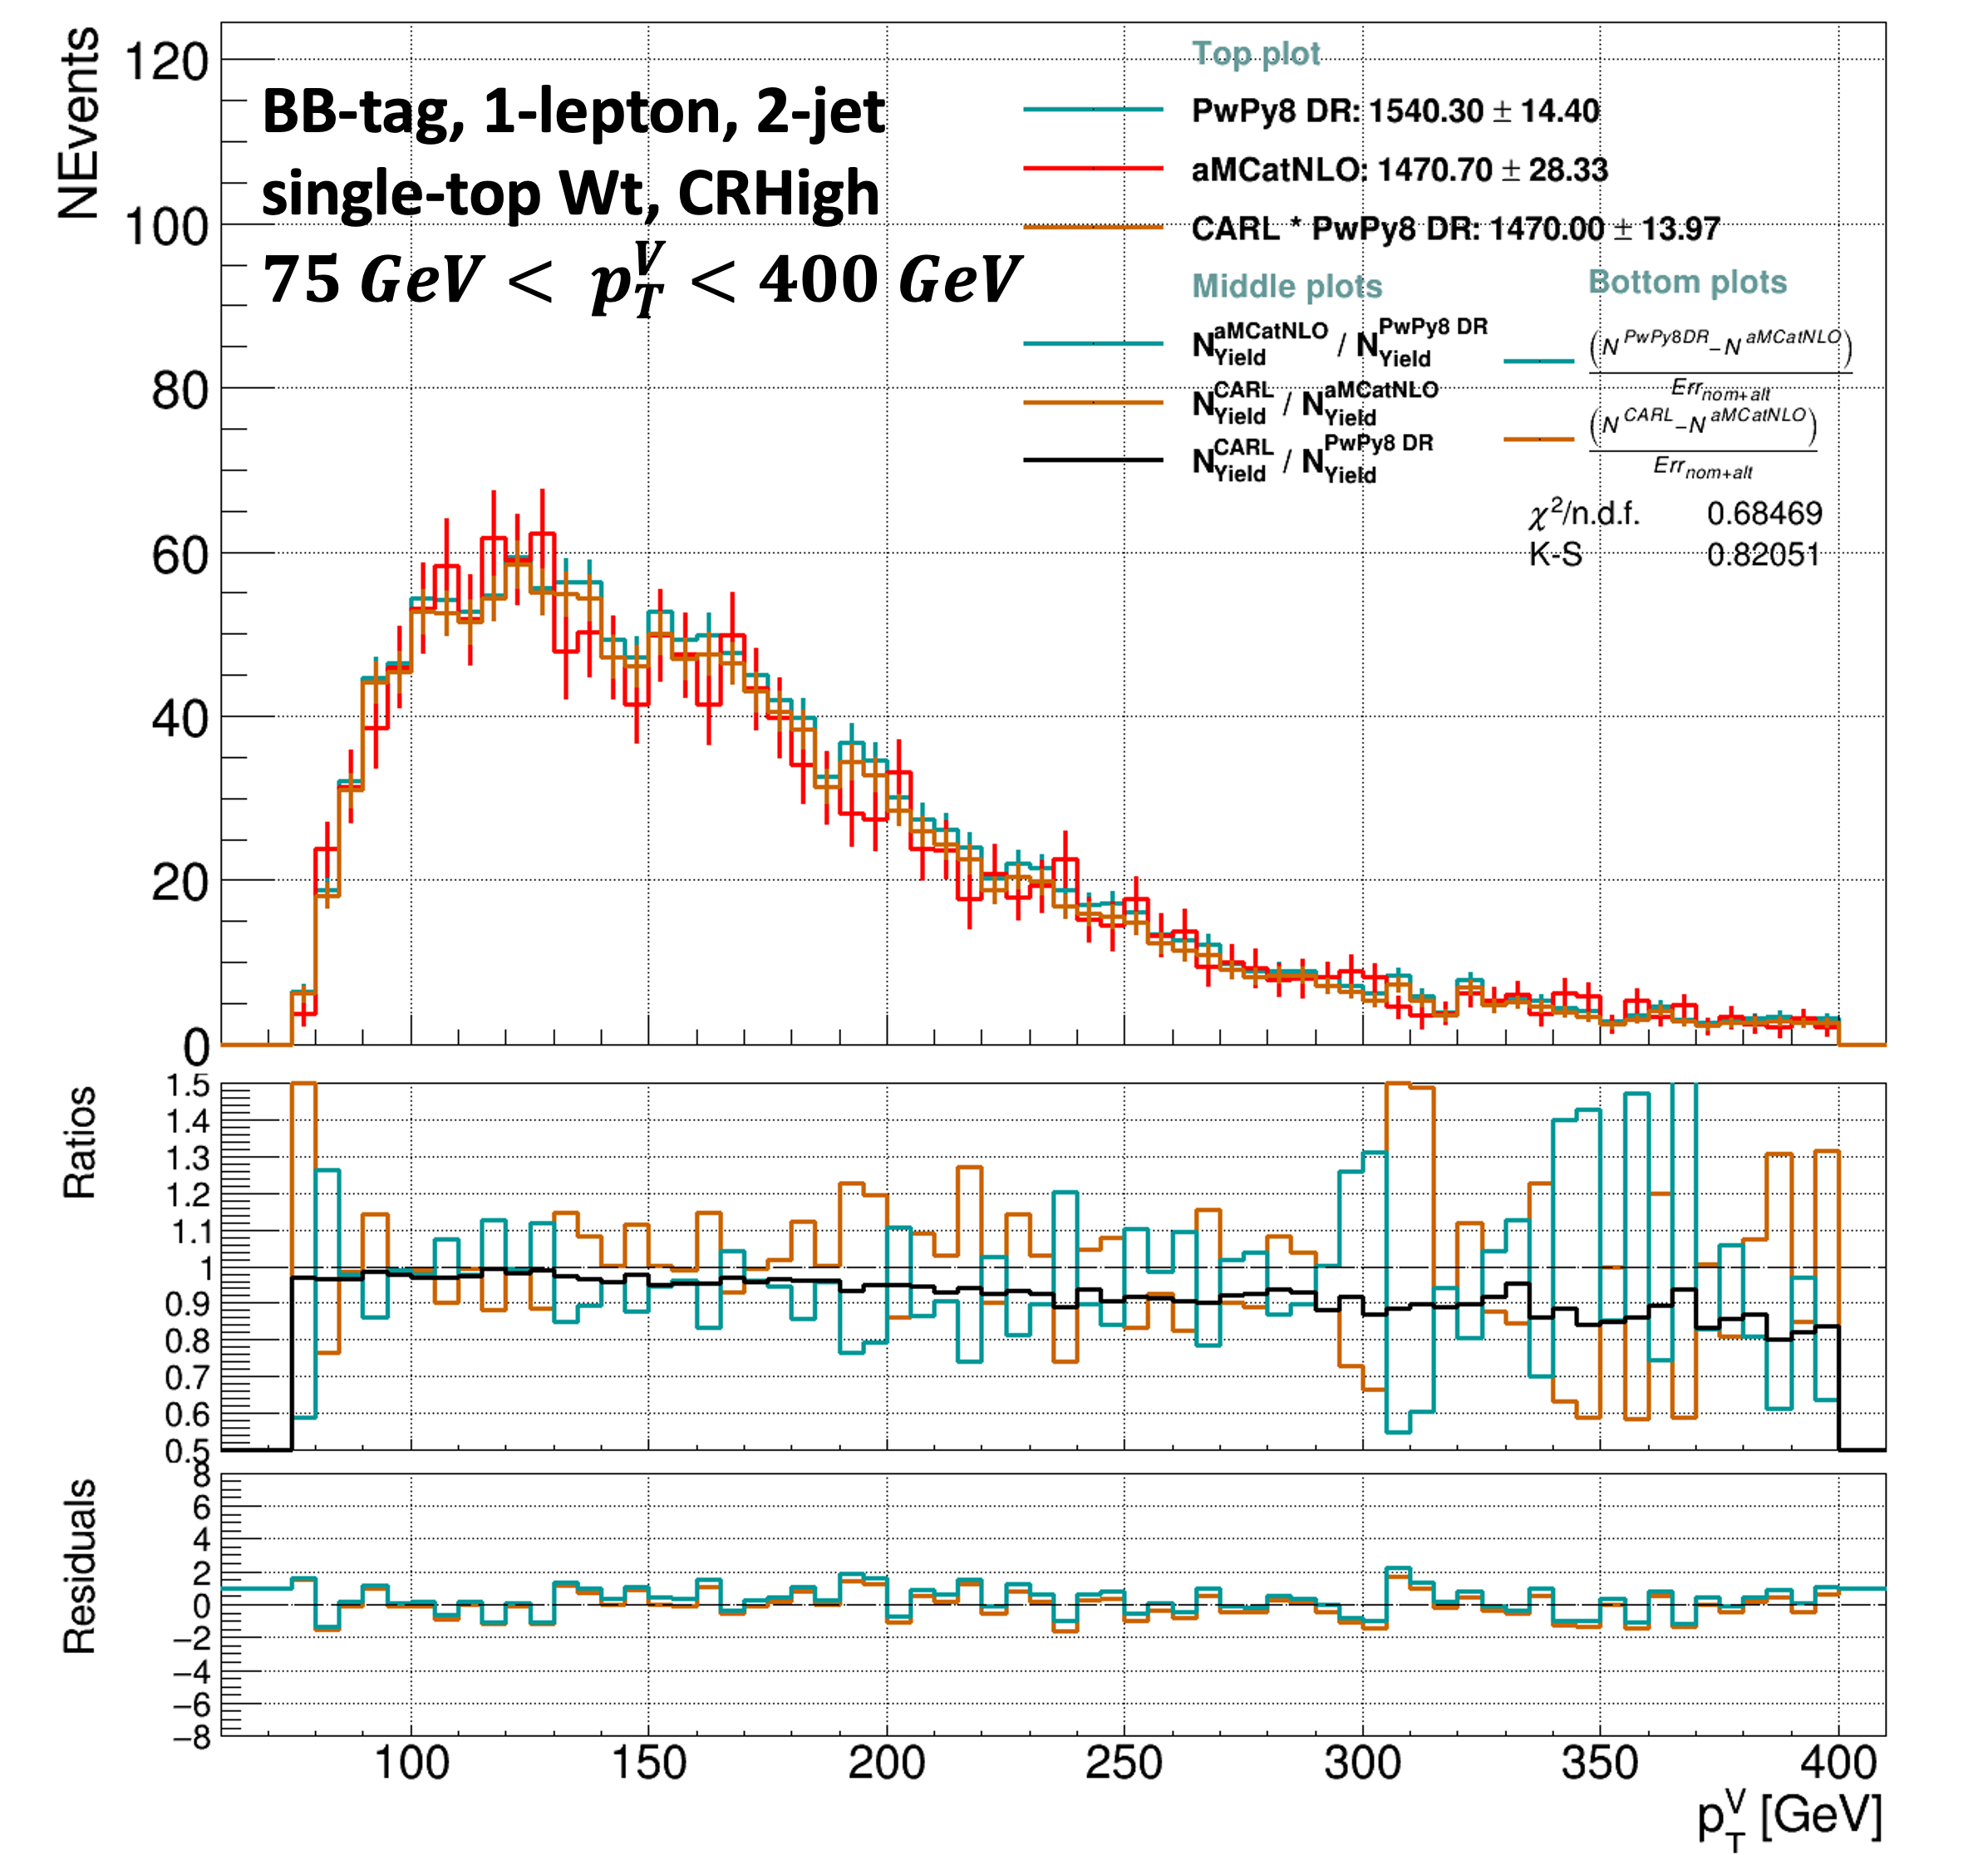
\includegraphics[width=0.48\textwidth]{Images/VH/Carl/wt/crhigh.png}
      }
      \caption{CARL closure plots, between the nominal \textsc{Powheg}\textsc{Pythia}8 (\textit{PwPy8}, with the DR scheme) and the alternative \textsc{MadGraph5\_aMC@NLO} (\textit{aMCatNLO}), for the single-top $Wt$ production in \vhb, 1-lepton, 75 GeV < \ptv\ < 400 GeV, and 2 jets. The CARL interpolation (orange) of the nominal (blue) into the alternative (red) is smoother and with lower MC-stats. uncertainty. The top plots show the distributions, the middle plots the ratios, and the bottom plots the residuals.}
      \label{fig:carl:resolved_closure_stopWt}
  \end{figure}
  
\begin{table}
    \scriptsize
    \resizebox{\textwidth}{!}{
    \begin{tabular}{l c c}
        \hline \hline
        Uncertainties & Resolved \vhbc & Boosted \vhb \\
        \hline
        \textbf{Signal} \\
        $qqWH$ / $qqZH$ / $ggZH$ normalisation/acceptance & \multicolumn{2}{c}{Values from previous analyses \cite{ATLAS:2020fcp, ATLAS:2020jwz, Collaboration:2721696}} \\
        $H\to bb$ BR & \multicolumn{2}{c}{1.61\%} \\
        $H\to cc$ BR & \multicolumn{2}{c}{From +5.53\% to -1.99\%} \\
        \hline
        \textbf{$Z$+jets} \\
        $Z+$\textit{hf} normalisation & \multicolumn{2}{c}{Floating} \\
        $Z+$\textit{mf} normalisation & Floating & 35\% \\
        $Z+$\textit{lf} normalisation & Floating & 35\% \\
        $Z+$\textit{hf} flavour composition ratio & 8\% - 12\% & 6\% - 9\% \\
        $Z+$\textit{mf} flavour composition ratios & 4\% - 10\% & 6\% - 9\% \\
        High-$\Delta R$ CR to SR & 5\% - 30\% & - \\
        topCR-SR extrapolation ratio & - & 15\% - 25\% \\
        2L to 0L acceptance ratio & 2\% - 10\% & 3\%\\
        \ptv\ extrapolation & - & 15\% \\
        \hline
        \textbf{$W$+jets} \\
        $W+$\textit{hf} normalisation & \multicolumn{2}{c}{Floating} \\
        $W+$\textit{mf} normalisation & Floating & 36\% \\
        $W+$\textit{lf} normalisation & Floating & 38\% \\ % TODO in 1L < 150 GeV it's fixed at 25\% norm unc.
        $W+$\textit{hf} flavour composition ratios & 4\% - 25\% & 11\% \\
        $W+$\textit{mf} flavour composition ratios & 14\% - 29\% & 9\% - 15\% \\
        $W+$\textit{lf} flavour composition ratios & 9\% & - \\
        High / Low-$\Delta R$ CR-SR extrapolation ratios & 2\% - 63\% & - \\
        topCR-SR extrapolation ratio & - & 16\% - 27\% \\
        1L to 0L acceptance ratio & 3\% - 30\% & 20\% \\
        \ptv\ extrapolation & - & 3\% \\
        $N_{\mathrm{jet}}$ extrapolation & 12\% - 20\% & - \\
        \hline
        \textbf{Top (\ttb\ + single-top $W$t) 0L \& 1L resolved} \\
        Top$(bb)$ normalisation & Floating &  - \\
        Top$(bq/qq)$ normalisation & Floating & - \\
        Flavour acceptance ratios & 5\% - 10\% & - \\
        1L to 0L acceptance ratios & 2\% - 8\% & - \\
        High / Low-$\Delta R$ CR-SR extrapolation ratios & 2\% - 10\% & - \\
        $Wt$ / \ttb\ ratios & 12\% - 48\% & - \\
        \hline
        \textbf{Top (\ttb\ + single-top $W$t) 2L resolved} \\
        Normalisation in \vhc & Floating & - \\
        Normalisation in \vhb^* & 0.08\%   & - \\
        \hline
        \textbf{Single-top ($t$-channel) 0L \& 1L resolved} \\
        Normalisation $s$ - $t$ & 4.6\% - 17\% & - \\
        High / Low-$\Delta R$ CR-SR extrapolation ratios & 3\% - 17\% & - \\
        \ptv\ extrapolation ratios & 7\% - 15\%  & - \\
        \nj\ acceptance ratios & 15\% & - \\
        1L to 0L acceptance ratio & 6\% & - \\
        \hline
        \textbf{\ttb\ and single-top boosted} \\
        top (\ttb\ + $Wt$) normalisation & - & Floating \\
        single-top $s$ and $t$ normalisations & - & 4.6\% - 10\%\\
        1L to 0L acceptance ratio top & - & 6\% - 20\% \\
        topCR-SR acceptance ratio top & - & 10\%\\
        $Wt$ / \ttbar ratio & - & 22\% - 36\%
        \hline
        \textbf{Diboson} \\
        $WW$ / $ZZ$ / $WZ$ normalisation & 16\% / 17\% / 19\% &  16\% / 17\% / 27\%\\
        $ggVV$ normalisation & \multicolumn{2}{c}{30\%} \\
        Lepton channel acceptance & 2\% - 23\% & 7\% \\
        $N_{\mathrm{jet}}$ acceptance & 10\% - 30\% & - \\
        % VZ HP-LP acceptance & - & 10-15\% \\
        \ptv\ acceptance & 3\% - 16\% & 8\% - 40\% \\
        SR / CR acceptance & 6\% - 16\% & - \\
        STXS like binning acceptance & - & 1.2\% - 42.2\% \\ % TODO Need to find this for resolved
        \hline
        \textbf{Multi-jet (1L)$^*$} \\
        Normalisation & 20\% - 100\% & - \\
        \hline \hline
    \end{tabular}
    }
    \caption{Summary of the modelling systematic uncertainties considered. The values given refer to the size of the uncertainty affecting the yield of each background. Uncertainties in the shapes of the distributions are not
    shown but taken into account for all backgrounds. $^*$The multijet background in the 1L channel and the top background in the 2L $BB$-tagged resolved are data driven.}
    \label{tab:syst_summary}

\end{table}
 % TODO, need to check the signal uncertainties

An overview of the signals and backgrounds modelling systematics considered is presented in Figure \ref{tab:syst_summary}, with the full details listed in Appendix \ref{appsec-vh-backsigmod}. All uncertainties presented here are further processed before entering the fit. To remove large statistical fluctuations potentially present in shape systematics, these shapes are smoothed by iteratively rebinning the distribution until the statistical uncertainty in each merged bin of the nominal distribution is smaller than 5\%. When a systematic has a negligible impact on the distributions entering the fit, it is pruned away to ease convergence and reduce the fit complexity. This is applied to systematics causing a normalisation effect smaller than 0.5\% or when both the up- and down-variations have the same sign. Shape uncertainties are pruned if no bin in the distribution has a deviation above 0.5\% after the overall normalisation, or if only one of the up- or down-variation is non-zero. For very small background processes, both shape and normalisation uncertainties are pruned: if this is a signal-sensitive region - if the signal yield is > 2\% of the total in the region -, the uncertainties are pruned if the process is $\leq$ 2\% of the signal, while in non-signal sensitive regions the process must be $\leq$ 0.5\% of the total background. The rest of this section goes into the details of the modelling, highlighting some specificities and subtleties related to each process. 

\subsection{Signal Modelling}\label{sec-modSignal}
The three main signal productions $qq \rightarrow WH$, $q\bar{q} \rightarrow ZH$, and $gg \rightarrow ZH$ are modelled separately, with uncertainties addressing the production and the decay mode of the Higgs into $b\bar{b}$ or $c\bar{c}$. The goal of the analysis is to measure the fiducial cross-sections of the \vhb\ and the signal strength of the \vhc. This first objective is approached with the adoption of the \glsfirst{stxs} in the reduced scheme of stage 1.2 \cite{badger2016les, berger2019simplified}, depicted in Figure \ref{fig:model-stxsscheme}. The bins are defined in successive regions of transverse momentum of the vector boson \ptv, from truth information in the simulated samples, and the number of additional jets \nj\ in the event, at 0 or more than 1 additional jet.
  
  \begin{figure}[!htbp]
    \centering
    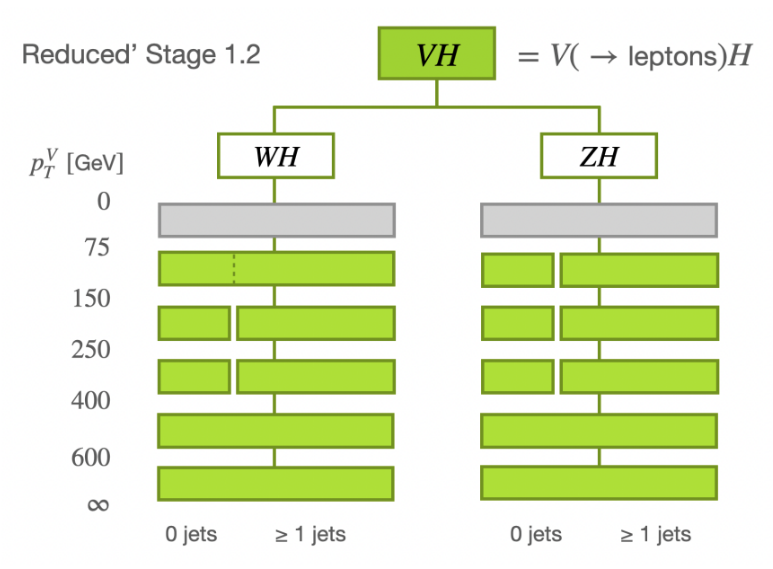
\includegraphics[width=0.58\textwidth]{Images/VH/Model/STXSsketch.png}
    \caption{The Standard Template Cross-Section scheme in the reduced stage 1.2 used for the combined \vhbc\ analysis.}
    \label{fig:model-stxsscheme}
  \end{figure}

The signal samples are finely binned following the \gls{stxs} prescription, with 5 \ptv\ bins for the $ZH$ covering $[75, 150[$ GeV, $[150, 250[$ GeV, $[250, 400[$ GeV, $[400, 600[$ GeV, and $\geq$ 600 GeV. The first three bins, corresponding to the resolved regime, are further split in \nj\ with 0 additional jet or $\geq 1$ jet, for a total of 8 different \glspl{poi} measured in $ZH$. For $WH$, the binning is similar to $ZH$ but there is no \nj\ splitting of the $[75, 150[$ GeV bin, giving a total number of 7 \glspl{poi} for $WH$. The full \gls{stxs} categorisation is used for \vhb\ and also for the \vhc, to enable correlation of the $VH$ uncertainties. For the \vhc\ however, the templates are merged and only one \gls{poi} is extracted: the global signal strength.\\
  
The signal is coherently modelled across the resolved and boosted regimes and targeted final state \vhb\ or \vhc. Several uncertainties are implemented to model the $VH$ production of the $H \rightarrow b\bar{b}/c\bar{c}$ decay. These uncertainties include:
\begin{itemize}
    \item \textit{\gls{qcd} scale uncertainties:} obtained by varying the renormalisation and factorisation scales $\mu_R$ and $\mu_F$. These variations are the most impactful in the theoretical prediction of the $VH$ production cross-sections. They are considered as shape uncertainties, implemented to cover modifications to the inclusive cross-sections and to parametrise possible migrations across \ptv\ and additional jet multiplicity bins, following Ref \cite{ATL-PHYS-PUB-2018-035}. The quark- and gluon-initiated signal processes have cross-section modifications parametrised separately. 
    \item \textit{\gls{pdf} + $\alpha_s$ uncertainties}: alternative parton distributions from the \textsc{PDF4LHC15\_30} modifying the $VH$ cross-sections in \gls{stxs} bins are considered  \cite{Butterworth:2015oua}. The $VH$ cross-sections in each \gls{stxs} bin are systematically modified by comparing the nominal \gls{pdf} to 30 alternatives. Furthermore, the $\alpha_s$ estimated at the $Z$-mass is varied for the nominal setup within its uncertainties. These uncertainties are separately calculated for $qq$-initiaded $WH$ and $ZH$, and for $gg$-initiated $ZH$. Shape effects on the resolved regime \ptv\ distributions are considered, while variations to the boosted large-$R$ mass $m_J$ and the invariant mass $m_{bb}$ or $m_{cc}$ are negligible.
    \item \textit{\gls{ew} corrections}: NLO electroweak corrections from NNLO \gls{ew} effects are considered with uncertainties modifying the \ptv\ distributions.
    \item \textit{Branching ratio}: a theoretical uncertainty of 1.61\% on the $H \rightarrow{b\bar{b}}$ branching ratio and an uncertainty covering the range from -1.99\% to +5.53\% for the $H \rightarrow{c\bar{c}}$ branching ratio are used \cite{LHCHiggsCrossSectionWorkingGroup:2016ypw}. The $ZH$ ($WH$) cross-sections cover 96.52\% to 104.11\% (97.95\% to 101.98\%) of their values thanks to additional uncertainties.
    \item \textit{Parton shower and underlying event uncertainties}: variations to the \gls{ps} and \gls{ue} can affect the properties of the $H \rightarrow b\bar{b} / c\bar{c}$ decays. Uncertainties are introduced to model these effects on signal acceptance. In the resolved regime, the effects of an alternative \gls{ps} model on the signal acceptance are evaluated on truth information in a similar phase space to the analysis selection. Acceptance uncertainties are derived by comparing the signal acceptance in the analysis categories between the nominal \textsc{Pythia} 8 and the alternative \textsc{Herwig} 7. Additional sub-leading acceptance uncertainties are evaluated by modifying the \textsc{Pythia} AZNLO tune. Differences in \ptv\ and $m_{bb}$ ($m_{cc}$) between \textsc{Pythia} and \textsc{Hewrig} are also considered, and the shape difference in the \gls{mva} distribution when adopting \textsc{Powheg}+\textsc{Herwig} 7 is used in the final stage of the analysis. In the boosted regime, the same strategy with the same \gls{ps} models is employed but the full detector response and event reconstruction are simulated, with uncertainties covering modifications to the $m_J$ distributions.
\end{itemize}

\subsection[$V+$jets Modelling]{$\boldsymbol{V+}$jets Modelling}\label{sec-modVjet} % TODO boosted
The $V+$jets processes are modelled separately for $Z+$jets and $W$+jets, depending on the flavour of the reconstructed vector boson. Their modelling nonetheless shares many similarities.

\subsubsection{$\boldsymbol{Z+}$jets}
This background is dominant in the 0L and 2L channels and limited in 1L. The background is split into different components from the flavour compositions of jets selected to form the Higgs candidate, grouping compositions with similar kinematic performance as:   
\begin{itemize}
    \item \textit{$Z+$ heavy flavours (\zhf)}: $Z+bb$ and $Z+cc$.
    \item \textit{$Z+$ mixed flavours (\zmf)}: $Z+bc$, $Z+bl$, and $Z+cl$.
    \item \textit{$Z+$ light flavours (\zlf)}: $Z+l$.
\end{itemize}
Each grouping has its own free-floating normalisations in 0L and 2L, with \zhf\ dominant in \vhb\ and the other two components significant in \vhc. These \glspl{fn} are decorrelated in \ptv\ and jet multiplicities \nj\footnote{Except for the 2L with 75 GeV < \ptv\ < 150, where the \vhb\ 4-jet is merged with 3-jet: to solve this, \vhb\ has an extra \zhf\ \gls{fn} for 3p-jet.}. The modelling of $Z+$jets includes several types of acceptance uncertainties that are applied only in 0L and 2L:
\begin{itemize}[leftmargin=*]
    \item \textit{Channel extrapolation 2L $\rightarrow$ 0L uncertainties}: for the \zhf, \zmf, and \zlf\ respectively. 
    \item \textit{Flavour composition uncertainties}: accounting for the variation on the yields of different flavours in the combinations with the double ratio of Equation \ref{eq-doubleRatio}. These include a ratio of $cc$ to $bb$ for \zhf, and of $bc$ and $bl$ to $cl$ for \zmf. They are decorrelated in \ptv\ and jet multiplicity \nj\ bins and cover the \vhb\ and \vhc\ sides of the resolved regime. 
    \item \textit{Region extrapolation uncertainties}: are included to model the acceptance of different regions, and derived with the double ratio Equation \ref{eq-doubleRatio} from a high purity region to a lower purity as:
    \begin{itemize}
        \item \zhf\ and \zmf: constrained mostly in the CRHigh and applied to the \gls{sr}. 
        \item \zlf: constrained mostly in 1 $LN$-tagged $V+l$ CR and the \gls{sr}, thus applied in CRHigh. % TODO, in the text, it says that it's SR - CRHigh, but it's constrained in LN??
    \end{itemize}
\end{itemize}
The values of the acceptance uncertainties are presented in Table \ref{tbl:zjets_acc_full} of Appendix \ref{appsec-vh-backsigmod}, with a summary mentioned in Table \ref{tab:summary_altsamples}. In addition, 4 different types of shape uncertainty are considered:
\begin{itemize}
    \item \gls{carl} shape: modelling the difference between \textsc{Sherpa} 2.2.11 and \textsc{MadGraph FxFx}, derived for all components and applied in all analysis regions.
    \item \textsc{Sherpa} 2.2.1 \ptv\ shape uncertainties to model the data-\gls{mc} mis-modelling of \ptv\ in \textsc{Sherpa} 2.2.11. The growing data-\gls{mc} disagreement with higher \ptv\ is visible in the plots of Appendix Figure \ref{fig:plots_VHcc_2L_TopCRemu}.
    \item \gls{qcd} scale shape uncertainties by varying $\mu_R$ and $\mu_F$.
    \item \gls{ew} shape variations that are typically quite small.
\end{itemize}  % TODO nothing about ISR / FSR?

\paragraph{Boosted regime:} the modelling strategy adopted is roughly the same as in the resolved regime, with the uncertainties fully detailed in the Appendix Table \ref{tbl:zjets_acc_fullBoos}. The \zhf\ component is left free-floating in 0L and 2L, while the \zmf\ and \zlf\ components both have overall acceptance uncertainties of 35\%. The \zlf\ has no other acceptance uncertainty since it is negligible in the boosted regime. Flavour acceptance uncertainties for \zhf\ and \zmf\ are applied in 0L and 2L. They also have channel acceptance uncertainties and \gls{sr} $\rightarrow$ Top CR acceptance ratios, both applied in the 0L. Additional \ptv\ extrapolation uncertainties from [400, 600] GeV to $> 600$ GeV are considered in 0L and 2L. Shape uncertainties are derived similarly to the resolved regime. 

\subsubsection{$\boldsymbol{W+}$jets}
This background is dominant in the 1-lepton channel, with a residual contribution in 0-lepton mostly due to hadronically decaying $\tau$-lepton. It is split equivalently to the $Z+$jets background as:   
\begin{itemize}
    \item \textit{$W+$ heavy flavours (\whf)}: $W+bb$ and $W+cc$
    \item \textit{$W+$ mixed flavours (\wmf)}: $W+bc$, $W+bl$, $W+b\tau$, $W+cl$, and $W+c\tau$.
    \item \textit{$W+$ light flavours (\wlf)}: $W+l$, $W+l\tau$, $W+\tau\tau$.
\end{itemize}
Each grouping has its own floating normalisation, with \whf\ significant in \vhb, while \wmf\ and \wlf\ are more important in \vhc. These \glspl{fn} are decorrelated in \ptv\ and jet multiplicities \nj\footnote{The only exception is the 1L \wlf\ in 75 GeV $<$ \ptv\ $<$ 150 GeV, where a normalisation uncertainty of 25\% is considered.}. Acceptance uncertainties, listed in the Appendix Table \ref{tbl:wjets_acc_full}, are applied in 0L and 1L. They include:
\begin{itemize}[leftmargin=*]
    \item \textit{Channel extrapolation 1L $\rightarrow$ 0L uncertainties}: applied in 0L for all components separately. 
    \item \textit{Flavour composition uncertainties}: include a comparison of $cc$ to $bb$ for \whf, of [$bc$, $bl$, $c\tau$, $b\tau$] to $cl$ for \wmf, and of [$l\tau$, $\tau\tau$] to $Wl$ for \wlf. They are decorrelated in \ptv\ and \nj, and cover the \vhb\ and \vhc\ sides. 
    \item \textit{Region extrapolation uncertainties} are defined differently for the combinations:
    \begin{itemize}
        \item \whf: constrained mostly in the \gls{sr} and the $BB$-tagged CRLow\footnote{\label{footnote-crlow}The CRLow is considered only in \vhb\ 1L.}, applied to CRHigh in different \ptv\ regions. For \vhb\ 1L, an extra CRLow $\rightarrow$ SR is applied. 
        \item \wmf: constrained mostly in 2 $c$-tagged CRHigh and applied to SR and CRLow\cref{footnote-crlow}.
        \item \wlf: constrained mostly in the SR and the 1 $LN$-tagged $V+l$ CR and applied in CRHigh. % TODO, in the text, it says that it's SR - CRHigh, but it's constrained in LN??
    \end{itemize}
    \item \textit{Jet multiplicity \nj\ acceptance}: \glspl{fn} are left free-floating in \nj\ (2-jet and 3-jet). For \vhb, the 4-jet category has no dedicated \gls{cr} and a 3-jet $\rightarrow$ 4-jet acceptance is applied to \whf\ (other components are negligible).
\end{itemize}
In addition, 4 different types of shape uncertainties are considered similarly to the $Z+$jets.

\paragraph{Boosted regime:} roughly the same modelling strategy is applied, with the uncertainties fully detailed in Appendix Table \ref{tab:wjets_acc_fullBoos}. The \whf\ component is left free-floating, while the \wmf\ and \wlf\ components have overall acceptance uncertainties of 36\% and 38\% respectively. Flavour acceptance uncertainties are considered for \whf\ from $bb$, and for \wmf\ from $bc$ (components with $\tau$ are negligible). The different components also have channel acceptance uncertainties applied in the 0L channel and \gls{sr} $\rightarrow$ Top CR acceptance ratios applied in the 0L and 1L channels. Additional \ptv\ extrapolation uncertainties from [400, 600] GeV to $> 600$ GeV are considered in 0L and 1L. Shape uncertainties are derived similarly to the resolved regime. 

\subsection{Top Modelling}\label{sec-modTop} 
The backgrounds including the decay of a top-quark $t$ are considered here, distinguishing between the \ttb\ pair-production and the single-top $Wt$ production as well as the single-top $t$- and $s$-channels, by decreasing order of relative importance. The \ttb\ and single-top $Wt$ are combined into a unified \textit{Top} component\footnote{Throughout this chapter, Top will refer to the combination of the \ttb\ \& $Wt$ processes.} in the resolved regime, and the single-top $t$- and $s$-channels are considered separately. The Top backgrounds in 0L and 1L are estimated from \gls{mc} and dedicated Top $BT$ control region, with the 2L case described later in this section. In the resolved regime, the Top is grouped into different components based on three truth flavour categories:
\begin{itemize}
    \item Top$(bb)$: which is mostly found in the \vhb\ phase space of the signal regions, and the \highdr\ \glspl{cr} thanks to the large initial angle between the emitted top-quark, passed over to the two $b$-quarks. 
    \item Top$(bq)$: combining top$(bc)$ and top$(bl)$. It is mostly in the \vhc\ phase space and is well-selected by the $BT$-tagged Top \gls{cr}.
    \item Top$(qq)$: combines top$(cc)$, top$(cl)$ and top$(ll)$, where $l$ is a light-jet ($u$, $d$, $s$, or a gluon). Mostly in the $TN$ and $TL$ regions of the \vhc. 
\end{itemize}

\begin{figure}[!htbp]
    \centering
      \subfloat[]{
        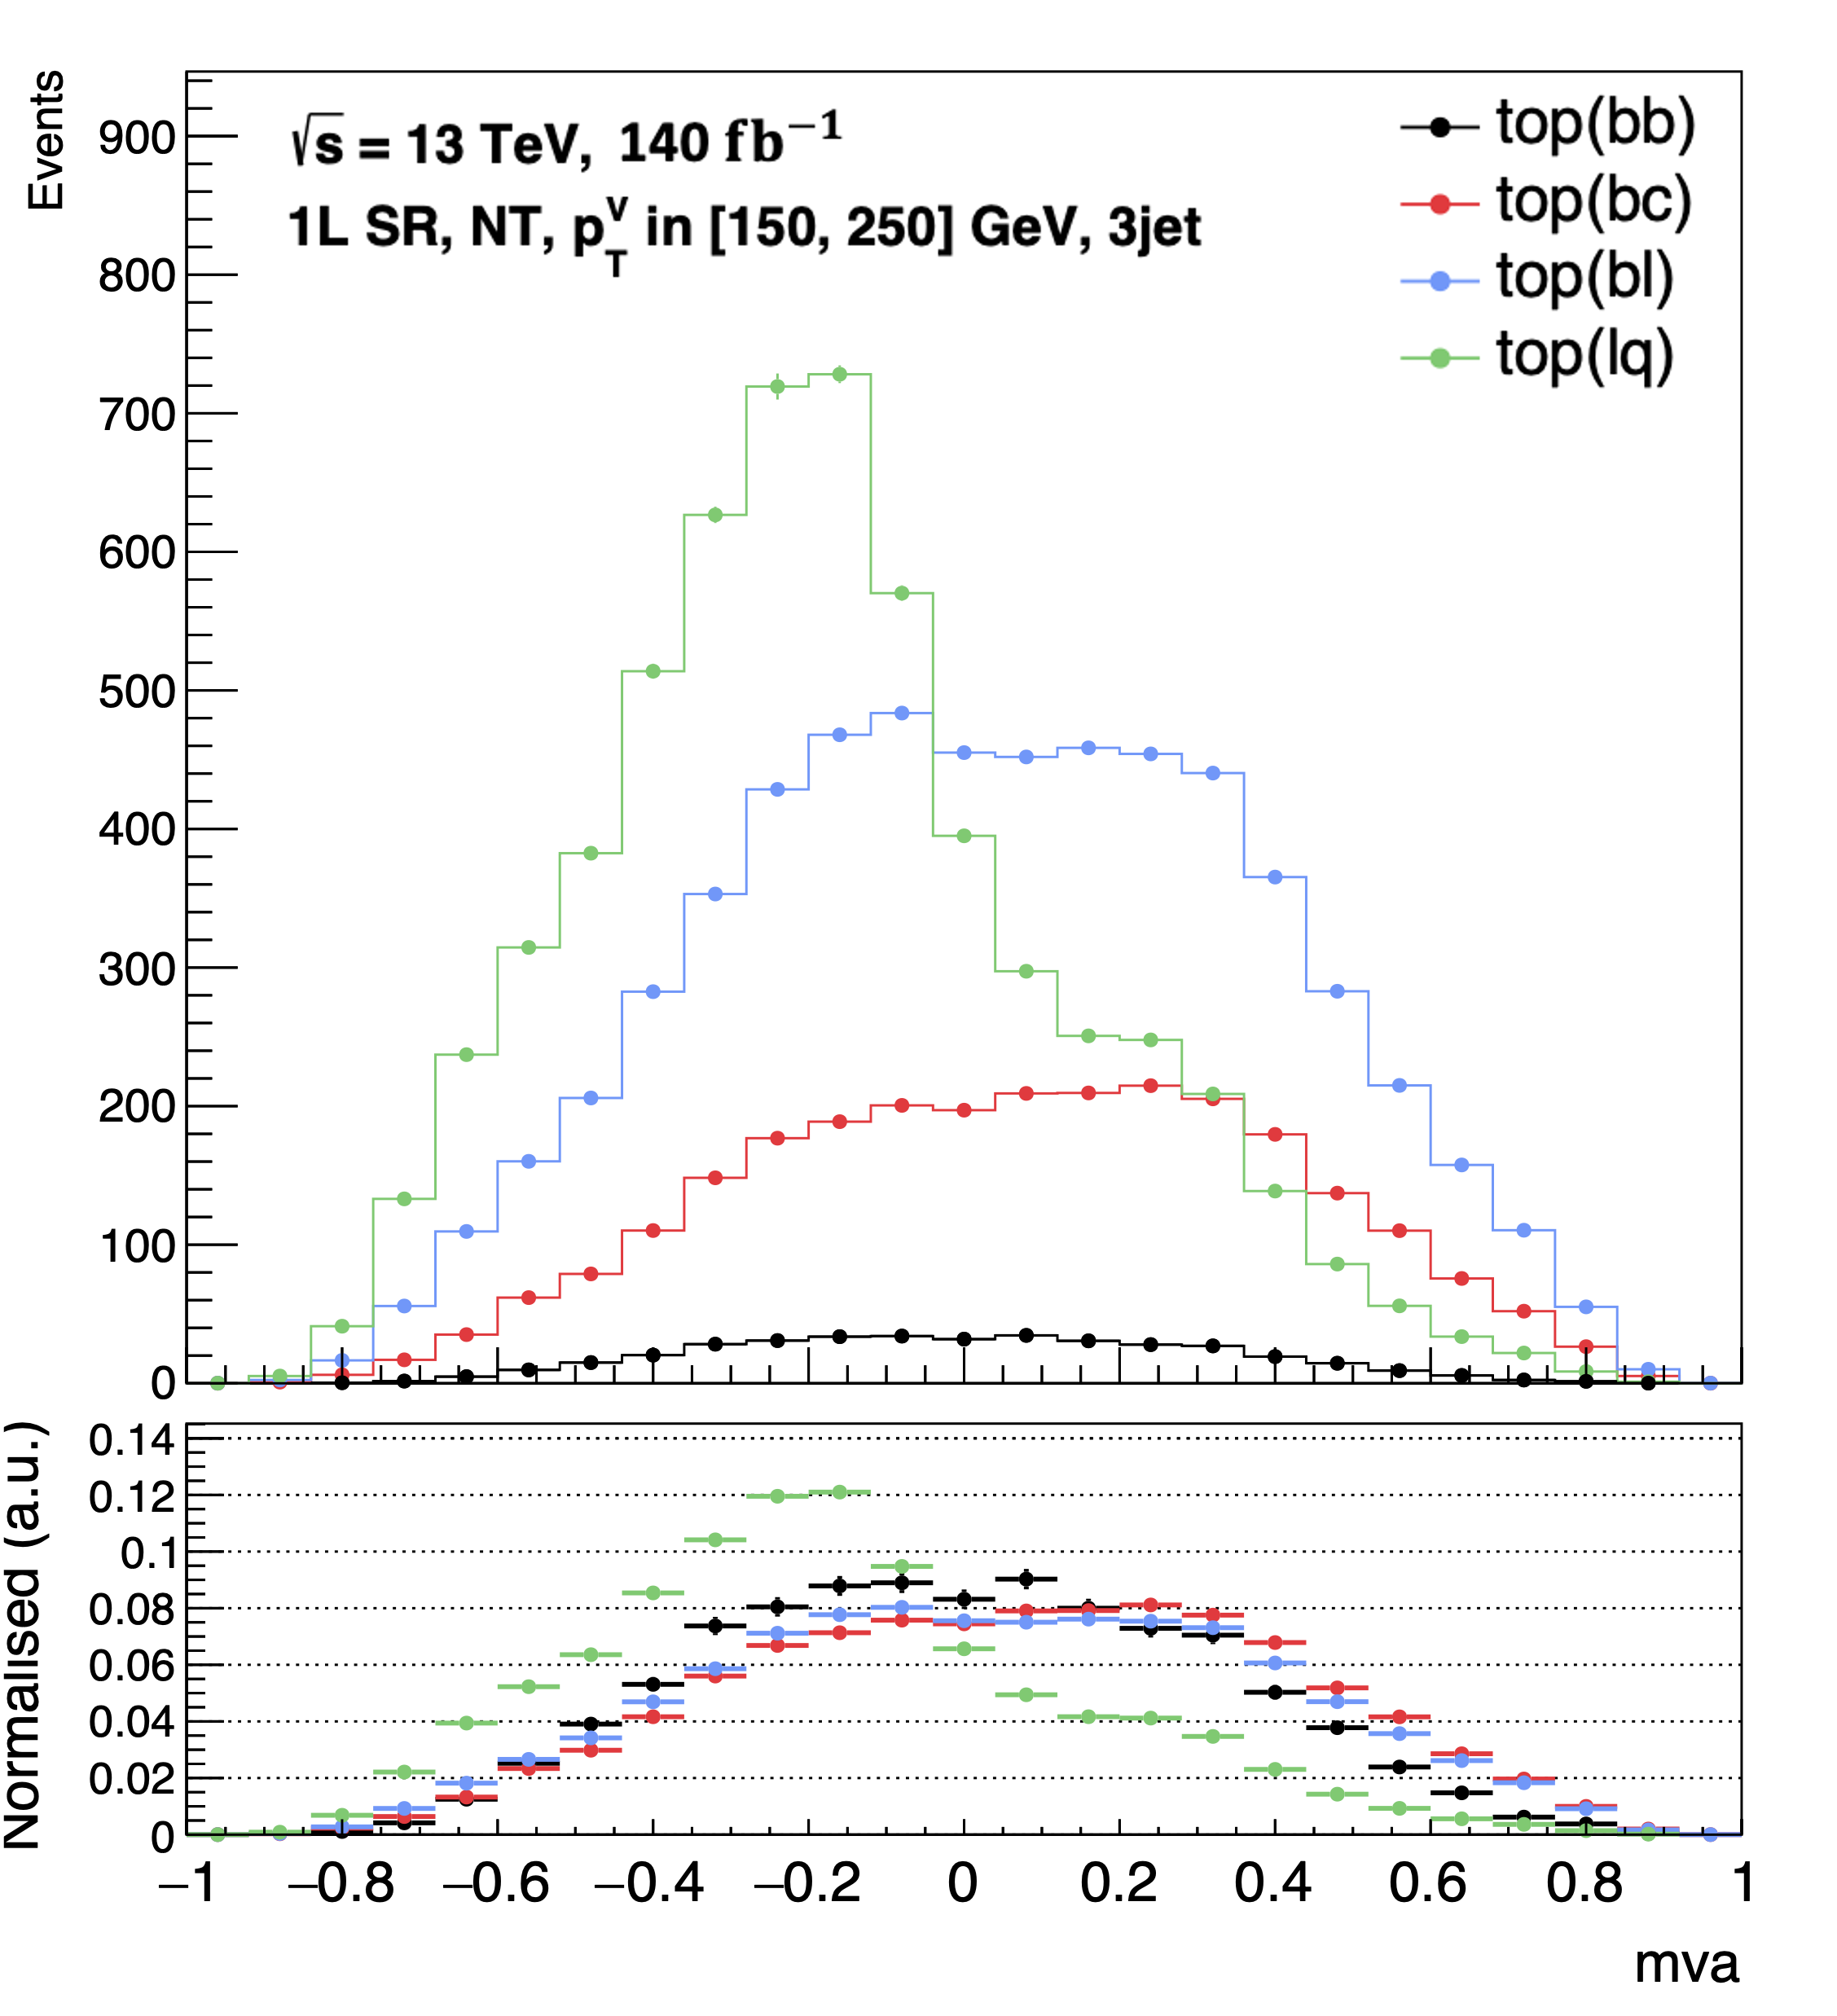
\includegraphics[width=0.45\textwidth]{Images/VH/Model/Top/TopcompoSRNT.png}
      }
      \subfloat[]{
        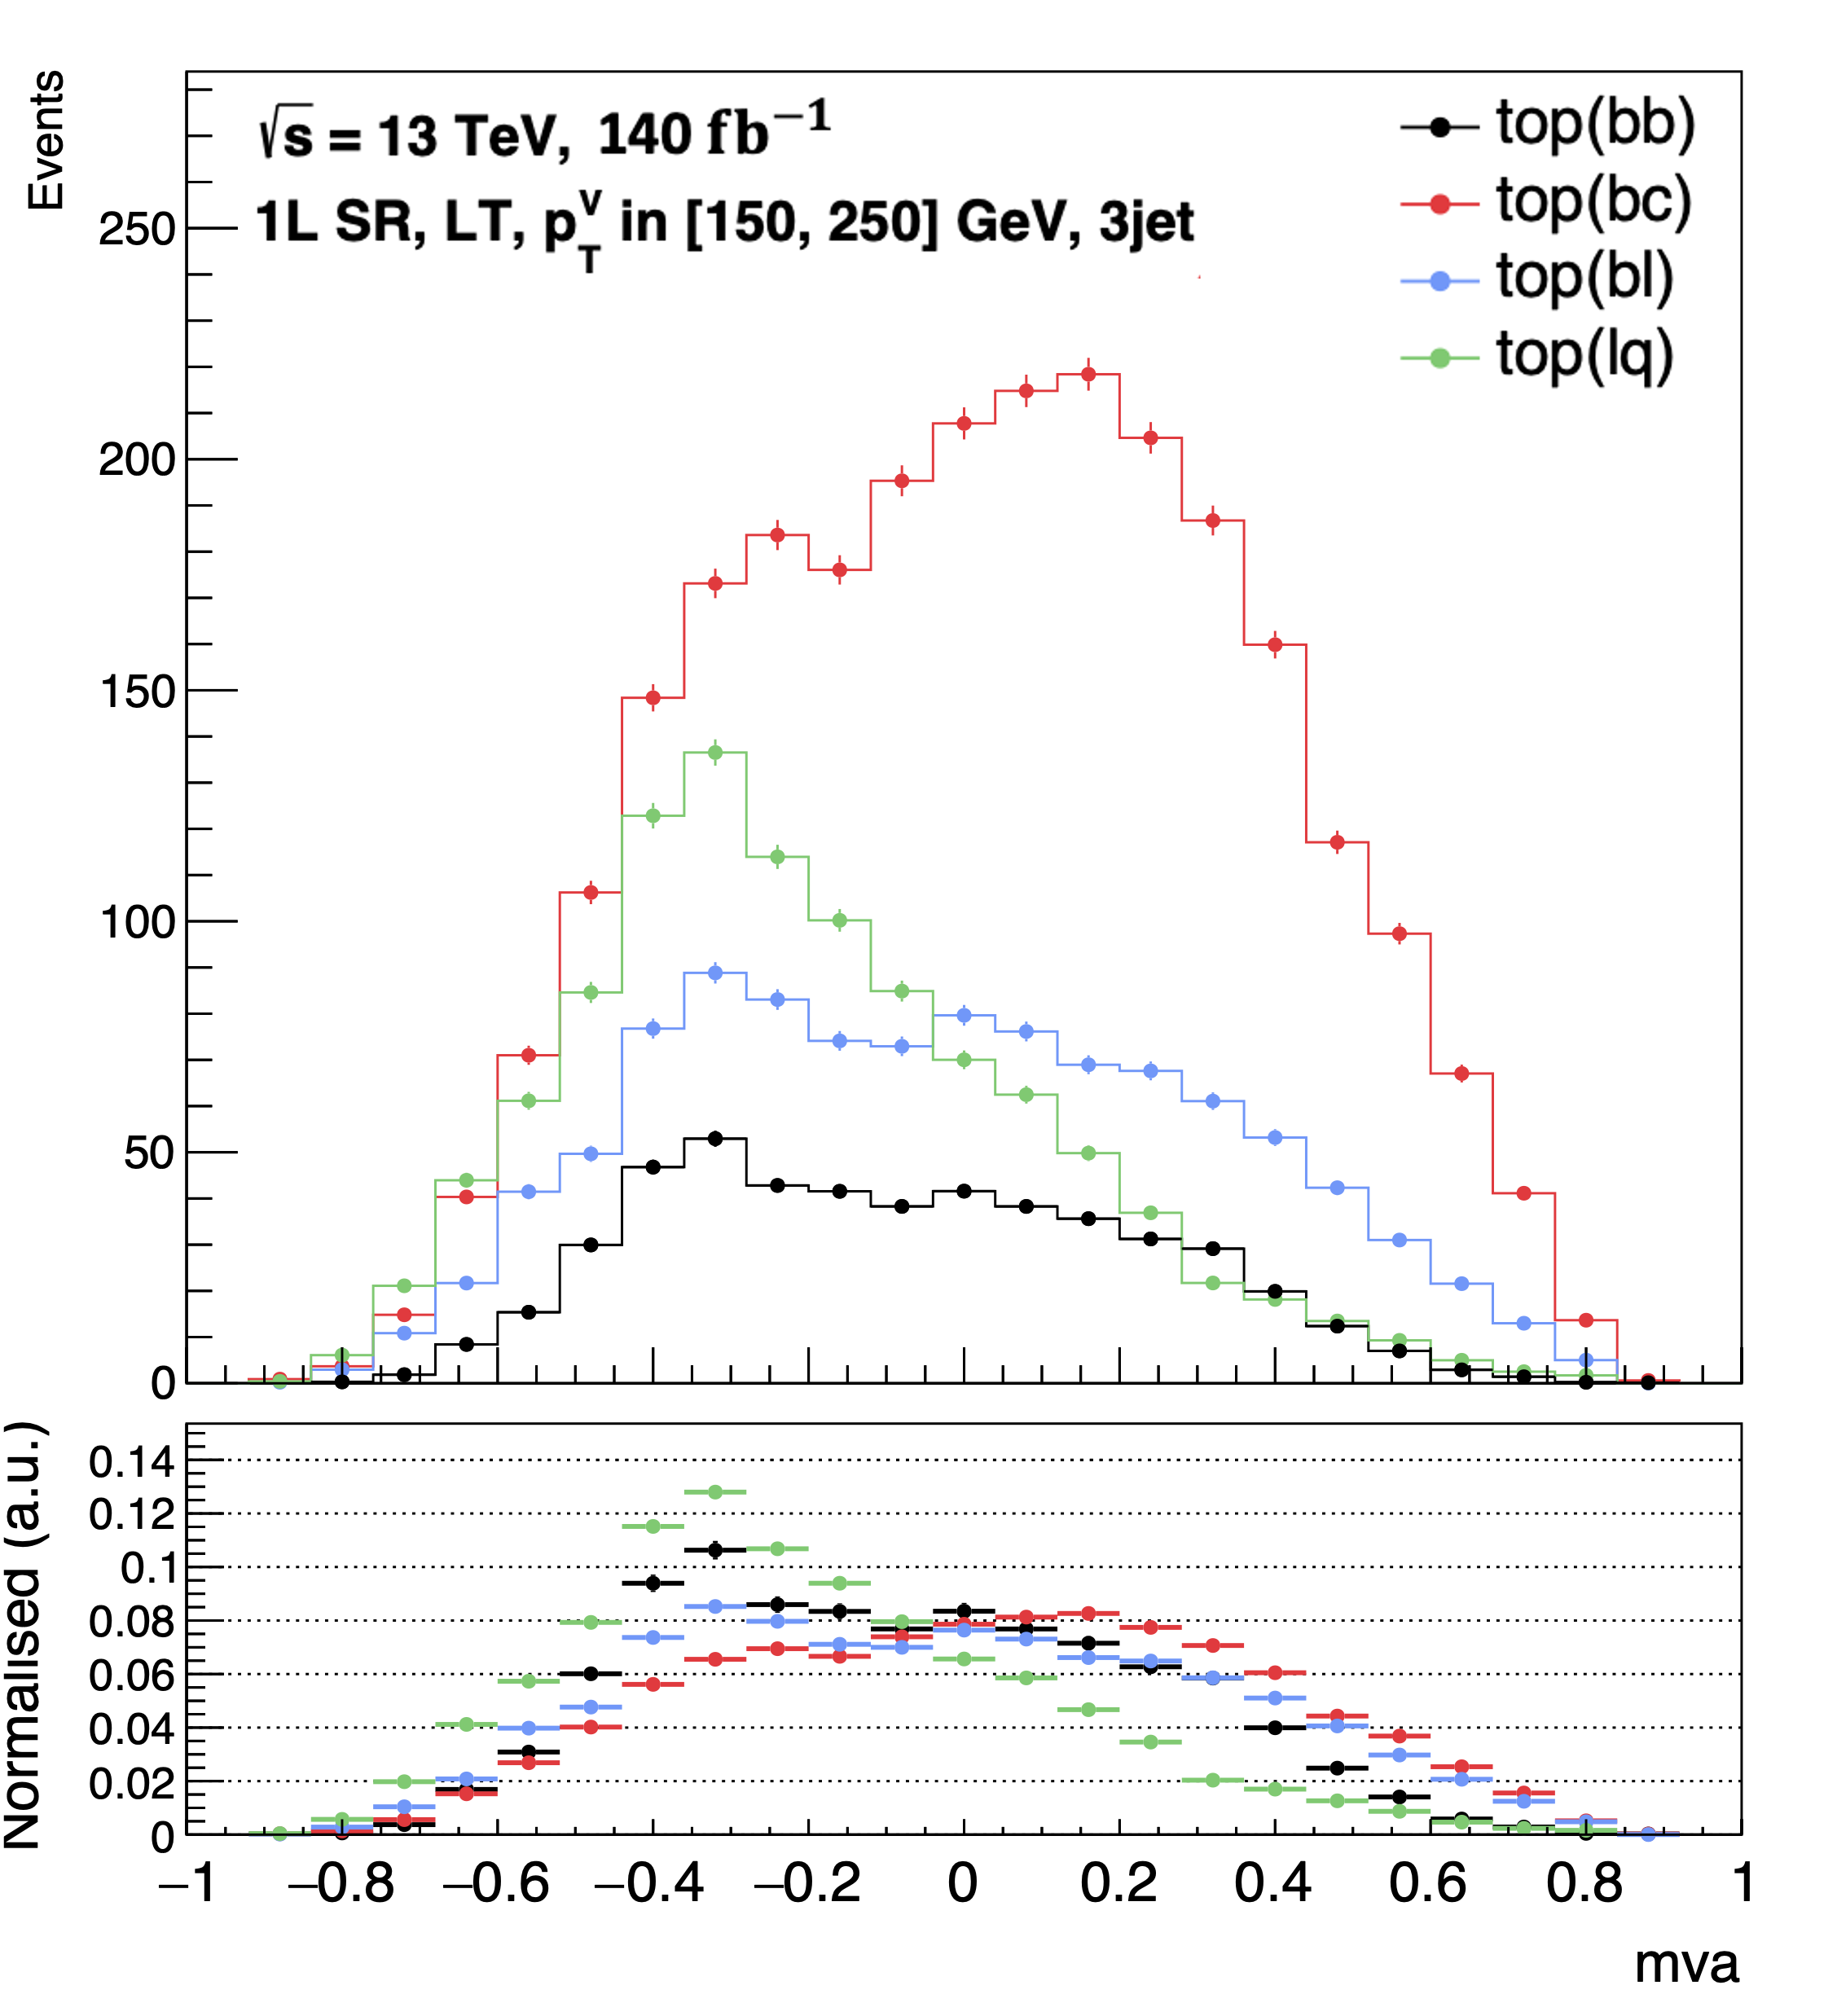
\includegraphics[width=0.45\textwidth]{Images/VH/Model/Top/TopcompoSRLT.png}
        }
      \caption{The non-rebinned MVA distributions of the top background components (direct tagged) in the \vhc\ signal regions ($TN$-tagged on the left, $TL$-tagged on the right) with 150 GeV $<$ \ptv\ $<$ 250 GeV and 3 jets. Top$(bb)$ in black, top$(bc)$ in red, top$(bl)$ in blue, and top$(qq)$ in green. The bottom panels show the normalised distributions.} 
      \label{fig:topflavdistr_VHcc}
\end{figure}

These groupings are based on the shared kinematics of the components, where the selected jets are either both $b$-jets and thus likely to directly come from the top-decays ($bb$), 1 $b$-jet likely from a top decay and 1 non $b$-jet from a subsequent hadronic $W$-decay or a radiated jet ($bc$ and $bl$, summarised $bq$), or neither directly from the top-decay ($cc$, $cl$, and $ll$, summarised $qq$). The $bc$ and $bl$ are combined into a single top$(bq)$ component as they indeed share the same kinematics, as illustrated in Figures \ref{fig:topflavdistr_VHcc} in the signal regions of \vhc\. This top$(bq)$ background is particularly significant in the \vhc\ analysis as it peaks at the signal mass (having a mass $\sim (m_{\text{top}} + m_W) / 2 \approx m_H$) and therefore exhibits signal-like properties such as reaching high MVA scores, as shown in Figure \ref{fig:topflavdistr_VHcc}. Due to the small contribution of the top$(qq)$ component, it is merged with the top$(bq)$ into a single top$(bq/qq)$ component, with the different sub-components shapes modelled by flavour composition uncertainties. The rest of this section details the modelling of the top backgrounds in the analysis regimes for 0L and 1L, followed by the single-top $t$- and $s$-channels in resolved, and finally the modelling adopted for the boosted regime.

\subsubsection{The $\boldsymbol{t\bar{t}}$ and $\boldsymbol{Wt}$ Resolved 0L \& 1L Modelling}
There are three main elements in the top background modelling scheme in the 0L and 1L resolved regime: floating normalisation, acceptance uncertainties, and shape uncertainties. On the first point, free-floating normalisations are applied for the top$(bb)$ and the top$(bq/qq)$ components, constrained respectively by the $BB$-tagged \highdr\ CR and the $BT$-tagged Top \gls{cr}. These \glspl{fn} are separated in jet multiplicity \nj\ (2-jet, 3-jet, and only for the 0L channel 4-jet) as well as \ptv, for a total of 16 \glspl{fn}. Concerning the second point, several types of acceptance uncertainties are applied, as summarised in Table \ref{tab:summary_altsamples} and detailed in the Appendix Table \ref{tab:top_summary}:
\begin{itemize}[leftmargin=*]
    \item \textit{Channel extrapolation 1L $\rightarrow$ 0L uncertainties}: the Top is dominant in 1L, hence the \glspl{fn} derivation is driven by the 1-lepton channel and applied to the 0-lepton one. This uncertainty is split in \ptv: 2\% in [150, 250] GeV and 8\% in [250, 400] GeV.
    \item \textit{Flavour composition uncertainties}: the top$(bq/qq)$ includes differently shaped sub-components. Uncertainties are derived from the alternative samples with the double ratio Equation \ref{eq-doubleRatio}, comparing $bl$ and $qq$ to $bc$ (of 5\% and 10\% respectively). 
    \item \textit{Region extrapolation uncertainties}: the top$(bb)$ is dominant in the CRHigh while the top$(bq/qq)$ leads in the Top $BT$ \gls{cr}, hence the extrapolations differ for the components. They are all derived from the double ratios with alternative samples.
    \begin{itemize}
        \item Top$(bb$): extrapolation uncertainties are derived from the CRHigh and applied in the \gls{sr}, the Top \gls{cr} and the CRLow\cref{footnote-crlow}. Additional uncertainties are applied from the \gls{sr} to the Top \gls{cr} and CRLow\cref{footnote-crlow}. All uncertainties are split per \ptv.
        \item Top$(bq/qq)$: the uncertainties are derived from the \gls{sr} + Top \gls{cr} + CRLow\cref{footnote-crlow}, due to their shared kinematic, and applied to the CRHigh. Additional uncertainties are applied from the \gls{sr} and Top \gls{cr} to the CRLow\cref{footnote-crlow}. All uncertainties are split per \ptv.
    \end{itemize}
    \item \textit{Process acceptance ratios}: in the \ttb\ and $Wt$ combination, the \ttb\ dominates and drives the normalisation. Additional acceptance uncertainties are included and applied to the $Wt$ to model differences in the relative contributions of the two processes. These are calculated with a double ratio in the different \ptv\ regions, lepton channels, and flavour components. They range from 12\% to 48\%.
\end{itemize}
In addition, several different shape uncertainties are considered for the Top backgrounds: 
\begin{itemize}
    \item \gls{carl} shapes: modelling the difference between the nominal samples (\textsc{Powheg}+\textsc{Pythia} 8) and the alternative modelling of the parton shower (\textsc{Powheg}+\textsc{Herwig} 7) and matrix element (\textsc{MadGraph5\_aMC@NLO}+\textsc{Pythia} 8). These \gls{carl} models are trained separately for \ttb\ and $Wt$ and per lepton channel, inclusively in flavour compositions and \nj. The DR scheme is used as nominal for these training of $Wt$ because the alternative samples use the same \ttb\ overlap removal scheme. 
    \item A DS-DR shape uncertainty is derived uniquely for $Wt$ to account for possible shape effects from modifications to the overlap removal procedure with \ttb. The \textsc{Powheg}+\textsc{Pythia} 8 samples with DS scheme are directly used in the fit as templates, thanks to their sufficient statistics. This shape uncertainty is unique in the combined analysis: it simultaneously applies a normalisation uncertainty, to account for the different yields of the DS- and DR-schemes.
    \item \gls{isr} and \gls{fsr} shape uncertainties are derived by varying the scales $\mu_R$ and $\mu_F$ from the nominal setup. For both, an up- and a down-variation are considered, with the variations being symmetric for the \gls{isr} while the down-variation of \gls{fsr} is smaller than the up-variation. % TODO treatment of symmetrised not clear.
\end{itemize} 

\subsubsection{The Single-Top $\boldsymbol{t}$- \& $\boldsymbol{s}$-channels in Resolved 0L \& 1L Modelling}
The single-top $t$- and $s$-channels are almost negligible in the analysis, except in the \vhb\ resolved at low \ptv, where the $t$-channel reaches a total backgrounds fraction of $\sim$8\% in the 1L 75 GeV < \ptv\ < 150 GeV. The importance of single-top $t$ quickly reduces with increasing energy\footnote{Except in the CRHigh region where the ratio stays in the 7\%-9\% range.}. In 0L and 1L, the single-top $t$- and $s$-channels are only applied cross-sections uncertainties of 17\% and 4.6\%, respectively. The single-top $t$-channel has several additional acceptance uncertainties derived by double ratio computations with alternative samples to model: 
\begin{itemize}
    \item \textit{channel extrapolation uncertainty}: of 6\% from 1L to 0L.
    \item \textit{Region extrapolations uncertainties}: depends on the \ptv. For \ptv\ < 150 GeV, the uncertainty is applied from SR $\rightarrow$ CRLow+CRHigh, with an additional CRHigh $\rightarrow$ CRLow uncertainty in 1L. For the higher \ptv\ regions, the extrapolations are instead from CRHigh $\rightarrow$ SR+CRLow\cref{footnote-crlow}, with an additional SR $\rightarrow$ CRLow\cref{footnote-crlow} uncertainty, due to the higher purity of the CRHigh.
    \item \textit{Jet multiplicity extrapolations}: are considered from the 3-jet to the 2-jet, and from the 2+3-jet to the 4-jet in 0L.
    \item \textit{\ptv\ extrapolation uncertainties}: since the single-top $t$-channel is mostly present in the lowest \ptv\ regions, \ptv\ extrapolation uncertainties are included from [75, 150] GeV to [150, 400] GeV, with an additional [150, 250] GeV to [250, 400] GeV uncertainty.
\end{itemize}
In addition, \gls{carl} and \gls{isr}/\gls{fsr} shape uncertainties are considered for the single-top $t$-channel in 1L only, as is done for the Top background. Table \ref{tab:stopt_summary} of the Appendix details the various single-top uncertainties considered.

\subsubsection{Resolved Regime Top Backgrounds in 2L} 
For the 2L \vhb\ resolved, data-driven estimates are used, deriving a template in the Top $e\mu$ region for the Top background with an 0.8\% extrapolation uncertainty to the signal region. For \vhc, the Top $e\mu$ region is used as a control region with the Top background left free-floating.

\subsubsection{Boosted Regime Top Backgrounds} 
In the boosted regime, the \ttb\ benefits from a good Top \gls{cr} and is not combined with the $Wt$ in the presented results\footnote{Studies were, at the time of writing, ongoing to also merge these two processes in the boosted regime.}. The modelling in the boosted regime, detailed in the Appendix Tables \ref{tab:ttbar_summary_boosted} and \ref{tab:stopt_summary_boosted}, covers:
\begin{itemize}[leftmargin=*]
    \item \ttb: 1 \gls{fn} per \ptv\ region for 0L and 1L. In 2L, a 20\% normalisation uncertainty is applied. \textit{Channel extrapolation uncertainties} are derived from 1L $\rightarrow$ 0L, split per \ptv. Finally, \textit{region extrapolation uncertainties} of 10\% are applied in 0L and 1L from the boosted Top \gls{cr} to the \gls{sr}.
    \item Single-top $Wt$-, $t$-, and $s$-channels are not free floated but insead have respectively a 25\%, 10\%, and 4.6\% normalisation uncertainty. The $Wt$ has additional acceptance uncertainties, to cover the lepton channel extrapolation and a \ptv\ extrapolation from [400, 600] GeV to $>$ 600 GeV. 
\end{itemize}
In addition, boosted shape uncertainties are considered similarly to what is done in the resolved regime 0L and 1L.

\subsection{Diboson Modelling}
The diboson production background consists of the $WW$, $WZ$, and $ZZ$ processes. In \vhb, the $ZZ$ primarily contributes to the 2L channel, while $WZ$ with $W$ leptonically and $Z$ hadronically decaying contributes to the 1L. Both equally contribute to 0L. In \vhc, the main contributor to 2L is the $WZ$ with $W$ hadronically decaying for a $Z$ leptonically decaying, while in 1L it is the $WW$ process that contributes the most. Again, both contribute almost similarly to 0L. The resolved and boosted acceptance uncertainties are detailed in Table \ref{table:VV_Sys_Summary} and Table \ref{table:VV_SysBoos_Summary}. \\

In the resolved regime, the diboson processes are a small background in the analysis, so only normalisations uncertainties are used for $ZZ$ (17\%), $WW$ (16\%), and $WZ$ (19\%) for the $qq$-initiated, and $ggVV$ (30\%) for the $gg$-initiated. All uncertainties are correlated between \vhb\ and \vhc. The $VZ (\rightarrow b\bar{b})$ and $VZ (\rightarrow c\bar{c})$ are considered as signals of the cross-check analysis, and denoted as $VZbb$ and $VZcc$ in the diboson modelling. The rest of the $WW$, $WZ$, and $VZ$ are classified as background components, denoted as $VV$bkg. Acceptance uncertainties, summarised in Table \ref{tab:summary_altsamples} and detailed in the Appendix Table \ref{table:VV_Sys_Summary}. For the signal components, the uncertainties are split between the $ZZ$ and $WZ$ components and include:
\begin{itemize}[leftmargin=*]
    \item \textit{Channel extrapolation uncertainties}: two sets are considered due to the differences between the two components. One covers the 1L $\rightarrow$ 0L for $WZ$bb and $WZcc$, and the other the 2L $\rightarrow$ 0L for $ZZbb$ and $ZZcc$. They are split by \nj.
    \item \textit{Acceptance in jet multiplicity}: are considered from low (2-jet) to high jet-multiplicity. First to 3-jet, with a different value for the low \ptv\ region, then from 3-jet to 4-jet inclusively in \ptv\ for 0L and 2L. They are decorrelated between the different lepton channels.
    \item \textit{Region extrapolation uncertainties}: from the \gls{sr} to the CRHigh and CRLow\cref{footnote-crlow}, due to the higher diboson purity of the \gls{sr}, with an additional \gls{sr} to CRLow in \vhb\ 1L. These uncertainties are separated for the different lepton channels.
    \item \textit{\ptv\ extrapolation uncertainties}: the 150 < \ptv\ < 250 GeV region is the purest in signal diboson and is therefore used to extrapolate to the other \ptv\ regions, separately for the different lepton channels and \nj.
    \item \textit{\gls{stxs} binning acceptance uncertainties}: are included between \nj\ and \ptv\ regions for all $VZ$ signal diboson processes. They are modelled by \gls{qcd} scale variations. % TODO need to find this for resolved and put it in ModUncSum table.
\end{itemize}

For the background components\footnote{Thus excluding the signal-like $VZbb$ and $VZcc$ described above.} of $WW$, $W_{\text{had}}Z_{\text{lep}}$, $W_{\text{lep}}Z_{\text{had}}$, and $ZZ$, with the ``had'' or ``lep'' index specifying the type of decay of each boson, the acceptances uncertainties are similar to those of the signal components and include:
\begin{itemize}[leftmargin=*]
    \item \textit{Channel extrapolation uncertainties}: two sets covering 1L $\rightarrow$ 0L (for $WW$ and $W_{\text{lep}}Z_{\text{had}}$) and 2L $\rightarrow$ 0L (for $ZZ$bkg and $W_{\text{had}}Z_{\text{lep}}$) are included due to difference in purity.
    \item \textit{Acceptance in jet multiplicity}: go from low (2-jet) to high jet-multiplicity. First to 3-jet, with a different value for the low \ptv\ < 150 GeV region. Then from 3-jet to 4-jet inclusively in \ptv\ for 0L and 2L. They are derived separately for the different lepton channels. % TODO no value for the 4-jet?
    \item \textit{Region extrapolation uncertainties}: go from the \gls{sr} to the CRHigh, due to the higher diboson purity of the \gls{sr}, separately for the different channels.
    \item \textit{\ptv\ extrapolation uncertainties}: all extrapolation go from the 150 < \ptv\ < 250 GeV region to the other \ptv\ regions, due to the higher purity in diboson of the medium \ptv\ range, separately for the different channels.
\end{itemize}

In addition, the diboson processes are modelled with different shape uncertainties:
\begin{itemize}
    \item \gls{carl} shape uncertainties comparing the nominal \textsc{Sherpa} 2.2.11 samples to the two alternative samples \textsc{Powheg}+\textsc{Pythia}8 and \textsc{Sherpa} 2.2.1. The former accounts for differences to the matrix element and parton shower, while the latter accounts for the mis-modelled \ptv\ shape. These uncertainties are applied to all regions.
    \item \gls{qcd} scale shape uncertainties are included to model changes to the scales $\mu_R$ and $\mu_F$, similarly to the $V+$jets.
    \item \gls{pdf} shape uncertainties modelling variation to $\alpha_s$ are considered.
    \item \gls{ew} shape uncertainties are considered, similarly to $V+$jets.
\end{itemize}

\paragraph{Boosted regime:} is modelled similarly to the resolved regime, with the uncertainties fully detailed in Table \ref{table:VV_SysBoos_Summary} of the Appendix. Small contributions from misidentified $W$ decays as jets or mis-reconstructed leptons are taken into account. The $ZZ$ and $WZ$ have normalisation uncertainties of 17\% and 27\% respectively. Acceptance uncertainties considered cover the lepton channel acceptance, \ptv\ acceptance, and \gls{stxs}-like uncertainty covering the \ptv\ and \nj\ bins, as is done in the resolved regime.

\subsection{Multi-jet Modelling}\label{sec-modMultiJ} 
The multi-jet background is negligible in 0L and 2L and the boosted regime. In 1L, a data-driven estimate is used from a high-purity multi-jet control region obtained by inverting the lepton isolation requirements. Shapes are derived by a template fit on the $m_T^W$ distributions in the multi-jet \glspl{cr}. The shapes of the multi-jet are extracted to the \glspl{sr} of the resolved regime, primarily in \vhc, with extrapolation and normalisation uncertainties applied. Top and $W+$jets scale factors are applied to the template to account for the non-insignificant contributions of these processes in the multi-jet \glspl{cr}.